\chapter{Single variable derivatives} \label{single}

The goal in this chapter is to formalize derivatives of functions whose input is a single real number and whose output is also a single real number. Probably many aspects of this theory will be familiar to you from your first exposure to single variable calculus. While there will likely be more formality here than is typical of introductory calculus courses, I strongly encourage you to use the intuition you developed during your calculus course as you go through this chapter. 

\section{Two definitions of the derivative}

\subsection{Slope of the tangent line} \label{slope-of-tangent-line}

Let $S$ be a subset of $\R$ and $a \in S$ an interior point. We would like to define the tangent line to the graph of a function $f : S \to \R$ at $a$. Intuitively, the ``tangent line'' should be a line that ``just barely touches'' the graph of $f$ at the point $(a, f(a))$. But it's not immediately clear how to formalize this intuitive definition.  

One approach to formalization begins with noticing that this intuitive ``tangent line'' can be approximated by secant lines, and secant lines can be formalized without ambiguity. More precisely, for small values of $h$, the point $a+h$ is close to $a$ and still in $S$ since $a$ is an interior point of $S$. The slope of the secant line passing through the two points $(a, f(a))$ and $(a+h, f(a+h))$ is computed by the quantity
\[ \frac{f(a+h)-f(a)}{h}, \]
since the ``rise'' is $f(a+h)-f(a)$, and the ``run'' is $(a+h)-a = h$. This quantity is often called a \emph{difference quotient}\index{difference quotient}. See \cref{figure-difference-quotient}. 

\begin{figure}[ht]
	\begin{center}
	\begin{tikzpicture}
	\begin{axis}[
	xmin=-0.5,xmax=3,
	ymin=-0.5,ymax=2.25,
	ytick={0.7, 1.5},
	xtick={1,2},
	xticklabels={$a$, $a+h$},
	yticklabels={$f(a)$,$f(a+h)$},
	axis lines=middle,
	axis line style=lightgray,
	width=0.75\textwidth
	]
	\addplot[black,style=thick,<->] expression[domain=-0.5:2.45,samples=50]{(x*(x^2+1)+5)/10}; 
	
	
	\addplot[red,<->] expression[domain=0.5:2.4,samples=2]{0.8*(x-1)+0.7}; 
	
	
	\addplot[lightgray,dotted] expression[domain=0:2.75,samples=2]{0.7};
	\addplot[lightgray,dotted] expression[domain=0:2.75,samples=2]{1.5}; 
	\addplot +[mark=none,lightgray,dotted] coordinates {(1, 0) (1, 2)};
	\addplot +[mark=none,lightgray,dotted] coordinates {(2, 0) (2, 2)};
	
	\addplot[black,dashed] expression[domain=1:2,samples=2]{0.7}; 
	\addplot +[mark=none,black,dashed] coordinates {(2, 0.7) (2, 1.5)};
	
	\node[color=black,draw=black,circle,fill,inner sep=2pt] at (axis cs:1,0.7) {}; 
	
	\node[color=red,draw=red,circle,fill,inner sep=2pt] at (axis cs:2,1.5) {}; 
	\end{axis}
	\end{tikzpicture}
\end{center}
\caption{The graph of a function $f$ is depicted in black. The secant line passing through the two points $(a, f(a))$ and $(a+h, f(a+h))$ is depicted in red. The ``rise'' between these points is $f(a+h)-f(a)$, and the ``run'' is $h$. Thus the slope of the secant line is precisely the difference quotient $(f(a+h)-f(a))/h$.}  \label{figure-difference-quotient}
\end{figure}

As $h$ gets smaller and smaller, the secant line becomes a better and better approximation of our intuitive idea of the ``tangent line'' at $a$. So, we \emph{define} the slope of the tangent line to be the limit of the slopes of the secant lines. 

\begin{definition} \label{derivative-definition-single} \index{differentiable!differentiable at a point} \index{derivative!derivative at a point}
	A function $f : S \to \R$ is \emph{differentiable} at an interior point $a \in S$ if 
	\[ \lim_{h \to 0} \frac{f(a+h) - f(a)}{h} \]
	exists. If this limit does exist, its value is called the \emph{derivative of $f$ at $a$}. We will usually denote this derivative as $f'(a)$, but sometimes also as one of the following, where $x$ is the variable that is being used to denote the argument to $f$.  
	\[ \left.\frac{df}{dx}\right|_{x = a} \quad \frac{df}{dx} (a) \quad \left.\frac{d}{dx} f(x)\right|_{x = a} \] 
\end{definition}

\begin{exercise}
	Use the definition of the derivative to determine whether or not each of the following functions $f$ is differentiable at the given point $a$. If it is differentiable, calculate $f'(a)$. Check your answers by making sure they agree with geometric intuition and/or rules you learned during your introductory calculus course. 
	\begin{enumerate}[(a)]
		\item $f(x) = |x|$ at $a = 0$.
		\item $f(x) = x$ at $a = 0$. 
		\item $f(x) = x^2$ at $a = 0$. 
		\item $f(x) = x^2$ at $a = 2$. 
		\item $f(x) = \begin{cases} 1 & x \geq 0 \\ 0 & x < 0 \end{cases}$ at $a = 0$. 
		\item $f(x) = \begin{cases} rx & \text{if } x \geq 0 \\ sx & \text{if } x < 0 \end{cases}$ where $r \neq s$. 
	\end{enumerate}
\end{exercise}

\begin{exercise}[Power rule for positive integer exponents] \label{power-rule-positive} \index{power rule}
	Prove that, if $f(x) = x^n$ for a positive integer $n$, then $f'(x) = nx^{n-1}$ for all $x \in \R$. \begin{hint} Recall the binomial theorem, which says that
	\[ (x+h)^n = \sum_{k = 0}^n \binom{n}{k} x^k h^{n-k}. \]
	\end{hint}
\end{exercise}

\begin{exercise}[Constant functions rule] \label{constant-implies-derivative-zero-single}
	Prove that, if $f : S \to \R$ is \emph{constant}\index{constant function} (ie, there exists a real number $c$ such that $f(x) = c$ for all $x \in S$), then $f'(a) = 0$ for all interior points $a \in S$. 
\end{exercise}

\begin{exercise}[Differentiability implies continuity] \label{differentiable-implies-continuous-single}
	Prove that if $f : S \to \R$ is differentiable at an interior point $a \in S$, then $f$ is also continuous at $a$. 
\end{exercise}

\begin{exercise}
	Suppose $f : S \to \R$ is a function and $a \in S$ is an interior point. 
	\begin{enumerate}[(a)]
		\item If $f$ is differentiable at $a$, must it be the case that
		\[ f'(a) = \lim_{h \to 0} \frac{f(a+h)-f(a-h)}{2h} ? \]
		\item If 
		\[ \lim_{h \to 0} \frac{f(a+h)-f(a-h)}{2h} \]
		exists, must it be the case that $f$ is differentiable at $a$?
		\item What if we assume that 
		\[ \lim_{h \to 0} \frac{f(a+h)-f(a-h)}{2h} \]
		exists \emph{and} that $f$ is continuous at $a$? 
	\end{enumerate}
\end{exercise}

\begin{pedanticremark}
	You might wonder why definition \cref{derivative-definition-single} is only made for when $a$ is an interior point of the domain $S$. First of all, notice that \emph{at the very least} we need for $a$ to be a limit point of $S$. Indeed, if $a$ is not a limit point of $S$, then we cannot evaluate $f(a+h)$ for all sufficiently small values of $h$, so ``secant line'' stops making any sense at all. 
	
	The reason why we insist that $a$ be an interior point (rather than just a limit point) is a bit more subtle: requiring $a$ to be an interior point makes the definition resistant to changing the domain $S$. For example, suppose $S = [0,\infty)$ and $f : S \to \R$ is the function given by $f(x) = 1$ for all $x \in S$. Notice that $a = 0$ is a limit point but not an interior point of $S$. If we compute the limit
	\[ \lim_{h \to 0} \frac{f(0 + h)- f(0)}{h} \]
	in $S$, we find that it equals 0 (cf. your proof of  \cref{constant-implies-derivative-zero-single}). But suppose we ``extend'' the domain of the function $f$ to all of $\R$ by setting $f(x) = 0$ for all $x < 0$. Now the limit
	\[ \lim_{h \to 0} \frac{f(0 + h)- f(0)}{h} \]
	computed in $\R$ does \emph{not} exist (cf. \cref{differentiable-implies-continuous-single}). This means that we would have to talk about ``differentiability of $f$ with respect to $S$'' and ``the derivative of $f$ with respect to $S$.'' This is rather annoying, and insisting that $a$ be an interior point avoids this pedantry. More precisely, the assertion is that if $a$ is an interior point of $S$ and $S \subseteq T$ and $f : T \to \R$ is a function, then $f$ is ``differentiable with respect to $S$'' if and only if it is ``differentiable with respect to $T$,'' and ``the derivative of $f$ with respect to $S$'' equals ``the derivative of $f$ with respect to $T$.'' If you're still reading this pedantic remark, you should take a few minutes and prove this assertion. 
\end{pedanticremark}

\begin{unimportantremark}
	Occasionally, it's useful to talk about differentiability from just one side. Suppose $f : S \to \R$ is a function and $a \in S$ is an interior point. Then $f$ is \emph{left differentiable at $a$} if 
	\[ \lim_{h \to 0^-} \frac{f(a+h)-f(a)}{h} \]
	exists, and then the value of this limit is called the \emph{left derivative} of $f$ at $a$. Similarly, $f$ is \emph{right differentiable at $a$} if 
	\[ \lim_{h \to 0^+} \frac{f(a+h)-f(a)}{h} \]
	exists, and then the value of this limit is called the \emph{right derivative} of $f$ at $a$.
\end{unimportantremark}

\subsection{Best linear approximation}

Let's now reinterpret the definition of the derivative in a way that will be better suited to generalization to the multivariable setting in \cref{multi}. 

Suppose a function $f : S \to \R$ is differentiable at an interior point $a \in S$. As we saw in the previous section, the tangent line to the graph at the point $(a, f(a))$ is a line with slope $f'(a)$ passing through the point $(a, f(a))$. In other words, it is the graph of the function $t : \R \to \R$ given by
\[ t(x) = f'(a)(x-a) + f(a). \]
Since $t$ is ``close'' to $f$ near $a$, we should have that
\[ f(a+h)-f(a) \approx t(a+h) - t(a) = f'(a)h \]
for small values of $h$. See \cref{figure-linear-approximation}. 
\begin{figure}[ht]
	\begin{center}
		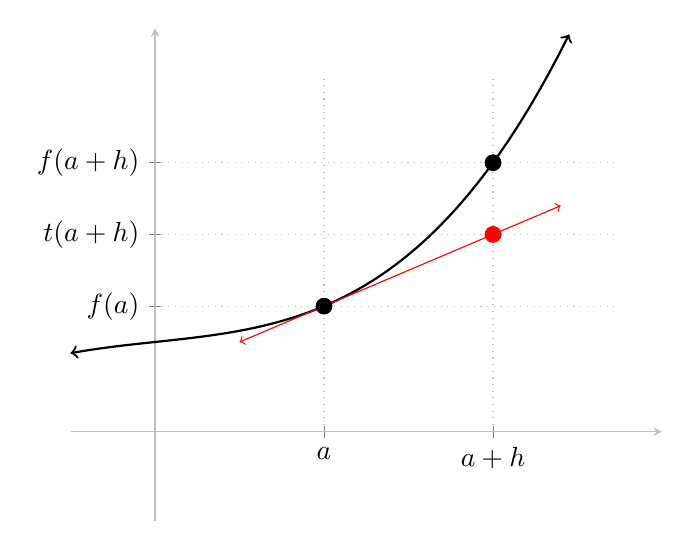
\begin{tikzpicture}
		\begin{axis}[
		xmin=-0.5,xmax=3,
		ymin=-0.5,ymax=2.25,
		ytick={0.7, 1.1, 1.5},
		xtick={1,2},
		xticklabels={$a$, $a+h$},
		yticklabels={$f(a)$, $t(a+h)$, $f(a+h)$},
		axis lines=middle,
		axis line style=lightgray,
		width=0.75\textwidth
		]
		\addplot[black,style=thick,<->] expression[domain=-0.5:2.45,samples=50]{(x*(x^2+1)+5)/10}; 
		
		
		\addplot[red,<->] expression[domain=0.5:2.4,samples=2]{0.4*x+0.3}; 
		
		
		\addplot[lightgray,dotted] expression[domain=0:2.75,samples=2]{0.7};
		\addplot[lightgray,dotted] expression[domain=0:2.75,samples=2]{1.1};
		\addplot[lightgray,dotted] expression[domain=0:2.75,samples=2]{1.5}; 
		\addplot +[mark=none,lightgray,dotted] coordinates {(1, 0) (1, 2)};
		\addplot +[mark=none,lightgray,dotted] coordinates {(2, 0) (2, 2)};
		
		\node[color=black,draw=black,circle,fill,inner sep=2pt] at (axis cs:1,0.7) {}; 
		\node[color=black,draw=black,circle,fill,inner sep=2pt] at (axis cs:2,1.5) {}; 
		\node[color=red,draw=red,circle,fill,inner sep=2pt] at (axis cs:2,1.1) {}; 
		\end{axis}
		\end{tikzpicture}
	\end{center}
	\caption{The graph of a function $f$ is depicted in black, and its tangent line $t$ at $a$ is depicted in red. Then the vertical distance $f(a+h)-f(a)$ is approximated by the vertical distance $t(a+h)-t(a)$. The ``rise'' $t(a+h)-t(a)$ can be computed as the slope times the ``run.'' In other words, $t(a+h)-t(a) = f'(a)h$. As $h$ gets smaller, this approximation of $f(a+h) - f(a)$ gets better.}  \label{figure-linear-approximation}
\end{figure}

Notice that the function $h \mapsto f'(a)h$ is a linear map $\R \to \R$, in the sense of linear algebra. The following result says that the function $h \mapsto f'(a)h$ is the \emph{only} linear map that is a good approximation\index{linear approximation} to $h \mapsto f(a+h)-f(a)$. The statement uses little-oh notation; if you have not seen this before, take a look at \cref{little-o-definition}.

\begin{proposition} \label{differential-unique-single}
	A function $f : S \to \R$ is differentiable at an interior point $a \in S$ if and only if there exists a linear map $\ell : \R \to \R$ such that
	\[ |f(a+h)-f(a) - \ell(h)| = o(|h|) \text{ as } h \to 0. \]
	Moreover, if there exists such a linear map $\ell$, then $\ell$ is uniquely determined: it must be given by \[ \ell(h) = f'(a)h \]
	for all $h \in \R$. 
\end{proposition}

\begin{proof}
	Let $\ell$ be a linear map $\ell(h) = ch$, where $c$ is some scalar. Observe that
	\[ \begin{aligned} \frac{|f(a+h)-f(a)-\ell(h)|}{|h|} &= \left| \frac{f(a+h)-f(a) - ch}{h} \right| \\
	&= \left| \frac{f(a+h)-f(a)}{h} - c \right|. \end{aligned} \]
	This leads us to the following sequence of ``if and only if'' statements. 
	\[ \begin{aligned} |f(a+h)-f(a)-\ell(h)| = o(|h|) &\iff \lim_{h \to 0} \frac{|f(a+h)-f(a)-\ell(h)|}{|h|} = 0 \\
	&\iff \lim_{h \to 0} \left| \frac{f(a+h)-f(a)}{h} - c \right| = 0 \\
	&\iff \lim_{h \to 0} \left( \frac{f(a+h)-f(a)}{h} - c \right) = 0 \\
	&\iff \lim_{h \to 0} \frac{f(a+h)-f(a)}{h} = c \end{aligned} \]
	The result follows. 
\end{proof}

\begin{definition}
	If $f : S \to \R$ is differentiable at an interior point $a \in S$, the \emph{differential} or the \emph{total derivative of $f$ at $a$}, denoted $df_a$, is the linear map $\R \to \R$ given by $df_a(h) = f'(a)h$. 
\end{definition}

Thus \cref{differential-unique-single} says that $df_a$ is the only ``good'' linear approximation to the function \[ h \mapsto f(a+h)-f(a). \] Since it is the only ``good'' linear approximation, it is also fair to say that it is the ``best'' linear approximation, whence the name of this section. The following is an important version of this same idea that comes up frequently in proofs. 

% TODO: add more here

\begin{remark}[Remainder function] \label{remainder-linear}
	Suppose $f : S \to \R$ is differentiable at an interior point $a \in S$. We define a remainder function\index{remainder} $r$ on sufficiently small values of $h$ by
	\[ r(h) = f(a+h) - f(a) - df_a(h). \]
	See \cref{figure-remainder-linear}. 
	\begin{figure}
		\begin{center}
			\begin{tikzpicture}
			\begin{axis}[
			xmin=-0.5,xmax=3,
			ymin=-0.5,ymax=2.25,
			ytick={0.7, 1.1, 1.5},
			xtick={1,2},
			xticklabels={$a$, $a+h$},
			yticklabels={$f(a)$, $f(a)+df_a(h)$, $f(a+h)$},
			axis lines=middle,
			axis line style=lightgray,
			width=\textwidth
			]
			\addplot[black,thick,<->] expression[domain=-0.5:2.45,samples=50]{(x*(x^2+1)+5)/10}; 
			
			
			\addplot[black,<->] expression[domain=0.1:2.4,samples=2]{0.4*x+0.3}; 
			
			
			\addplot[lightgray,dotted] expression[domain=0:2.75,samples=2]{0.7};
			\addplot[lightgray,dotted] expression[domain=0:2.75,samples=2]{1.1};
			\addplot[lightgray,dotted] expression[domain=0:2.75,samples=2]{1.5}; 
			\addplot +[mark=none,lightgray,dotted] coordinates {(1, 0) (1, 2)};
			\addplot +[mark=none,lightgray,dotted] coordinates {(2, 0) (2, 2)};
			
			
			\node[color=black,draw=black,circle,fill,inner sep=2pt] at (axis cs:1,0.7) {}; 
			\node[color=red,draw=red,circle,fill,inner sep=2pt] at (axis cs:2,1.5) {}; 
			\node[color=red,draw=red,circle,fill,inner sep=2pt] at (axis cs:2,1.1) {}; 
			
			
			\addplot +[mark=none,red,solid] coordinates {(2, 1.1) (2, 1.5)};
			\end{axis}
			\end{tikzpicture}
		\end{center}
		\caption{The thick black curve is the graph of a function $f$ and the thinner black line is its tangent line $f(a) + df_a$ are depicted in black. If $r$ is the remainder function, then $r(h)$ is the the vertical distance indicated in red above.}  \label{figure-remainder-linear}
	\end{figure}

	Notice that the $y$-value of the tangent line of $f$ at $a$ when $x = a+h$ is \[ f(a) + f'(a)h = f(a) + df_a(h), \]
	so $r(h)$ is what's left over after approximating $f$ by its tangent line (whence the name, ``remainder''). Notice that $r(0) = 0$. Moreover, $f$ is differentiable and therefore continuous at $a$ (cf. \cref{differentiable-implies-continuous-single}), so $r$ is also  continuous at 0. 
	
	Finally, the remainder function $r$ is ``small'' because $df_a$ is a ``good'' linear approximation of $f(a+h)-f(a)$. More precisely, we know from \cref{differential-unique-single} that $|r(h)| = o(|h|)$, which means that $r(h)/h \to 0$ as $h \to 0$. 
\end{remark} 

The following weak version of l'H\^opital's rule\index{lhopitals rule@L'H\^opital's rule} is an application of this idea. 
Note that this version of l'H\^opital's rule cannot be iterated (you cannot use it twice to evaluate $\lim_{x \to 0} (\sin x - x)/x^3$, for instance). In any case, in many cases it is often sufficient. 

\begin{exercise}[L'H\^opital's rule, weak version] \label{lhopital-weak}
	Suppose $f, g : S \to \R$ are differentiable at an interior point $a \in S$, that $f(a) = g(a) = 0$, and that $g'(a) \neq 0$. Show that
	\[ \lim_{x \to a} \frac{f(x)}{g(x)} = \frac{f'(a)}{g'(a)}. \]
	\begin{hint} 
		First show that, if $x = a+h$ and $r$ is the remainder function for $f$ defined in \cref{remainder-linear}, then
		\[ f(x) = f(a+h) = \left( f'(a) + \frac{r(h)}{h} \right)h. \]
	\end{hint}
\end{exercise} 

\section{Computing derivatives}

In this section, we'll prove some of the basic rules of differentiation that one normally encounters in an introductory calculus course. 

\subsection{Sum and scalar multiples rule}

The following results can be proved using either the definition of the derivative \ref{derivative-definition-single} or the ``best linear approximation'' characterization of \cref{differential-unique-single}. I strongly encourage you to try both methods for these exercises. 
When you use \cref{differential-unique-single}, you may find it useful to have done \cref{little-o-vector-space}. 

\begin{exercise}[Sum rule] \label{sum-rule-single} \index{sum rule}
	Prove that, if $f, g : S \to \R$ are both differentiable at an interior point $a \in S$, then $f + g$ is also differentiable at $a$ and \[ (f+g)'(a) = f'(a) + g'(a). \]
\end{exercise}

\begin{exercise}[Scalar multiples rule] \index{scalar multiples rule} \label{scalar-multiples-rule-single}
	Prove that, if $c$ is a constant and $f : S \to \R$ is differentiable at an interior point $a \in S$, then $cf$ is also differentiable at $a$ and \[ (cf)'(a) = c f'(a). \]
\end{exercise}

\begin{exercise}
	Suppose $f, g : S \to \R$ are functions and $f + g$ is differentiable at an interior point $a \in S$. Does it then follow that $f$ and $g$ are also differentiable at $a$? If so, prove it. If not, provide a counterexample. 
\end{exercise}

\subsection{Product and quotient rules}

\begin{proposition}[Product rule] \label{product-rule-single} \index{product rule}
	Suppose $f, g : S \to \R$ are both differentiable at $a \in S$. Then $fg$ is also differentiable at $a$ and 
	\[ (fg)'(a) = g(a) f'(a) + f(a)g'(a). \]
\end{proposition}

\begin{proof}
	The proof is a clever algebraic manipulation of difference quotients. The key trick is introducing a ``cross term'' of the form $f(a)g(a+h)$, and then cancelling it out by also introducing its negative. More precisely, for any sufficiently small real number $h$, we have 
	\[ \begin{aligned} \frac{(fg)(a+h)-(fg)(a)}{h} &= \frac{f(a+h)g(a+h) - f(a)g(a)}{h} \\ 
	&= \frac{f(a+h)g(a+h) {\color{blue}-f(a)g(a+h) + f(a)g(a+h)} - f(a)g(a)}{h} \\
	&= \frac{f(a+h)g(a+h) - f(a)g(a+h)}{h} + \frac{f(a)g(a+h) - f(a)g(a)}{h} \\
	&= g(a+h) \cdot \frac{f(a+h) - f(a)}{h} + f(a) \cdot \frac{g(a+h) - g(a)}{h}, \end{aligned} \]
	where the cross term and its negative is indicated in blue. 
	Taking the limit as $h \to 0$ yields the result. 
\end{proof}

\begin{exercise}
	Check your understanding of the above proof of the product rule. 
\begin{enumerate}[(a)]
	\item Could you have instead introduced a cross term of the form $f(a+h)g(a)$? If so, rewrite the proof using this cross term. If not, explain why not. 
	\item At what point is \cref{differentiable-implies-continuous-single} tacitly used in the above proof?
\end{enumerate}
\end{exercise}

\begin{exercise}
	 Reprove the scalar multiples rule (\cref{scalar-multiples-rule-single}) using the product rule. 
\end{exercise}

\begin{exercise}[Quotient rule] \label{quotient-rule-single} \index{quotient rule}
	Suppose $f, g : S \to \R$ are both differentiable at an interior point $a \in S$, and that $g(a) \neq 0$. Prove that $f/g$ is also differentiable at $a$ and 
	\[ (f/g)'(a) = \frac{g(a)f'(a) - f(a)g'(a)}{g(a)^2}. \] 
	\begin{hint} Observe that \[ \frac{(f/g)(a+h)-(f/g)(a)}{h} = \frac{\frac{f(a+h)}{g(a+h)} - \frac{f(a)}{g(a)} }{h}. \]
	Multiply both the numerator and denominator by $g(a+h)g(a)$ to clear the denominators inside the numerator, and then introduce the cross term $f(a)g(a)$. Be sure to notice at what point you use \cref{differentiable-implies-continuous-single}.
	\end{hint}
\end{exercise}

\begin{comment}
	Again, the proof is a clever algebraic manipulation of difference quotients! There are now two tricks: clearing denominators, and then introducing a cross term $f(a)g(a)$. 
	\[ \begin{aligned} \frac{(f/g)(a+h)-(f/g)(a)}{h} &= \frac{\frac{f(a+h)}{g(a+h)} - \frac{f(a)}{g(a)} }{h} \\ 
	&= \frac{g(a+h)g(a)}{g(a+h)g(a)} \cdot \frac{\frac{f(a+h)}{g(a+h)} - \frac{f(a)}{g(a)} }{h} \\
	&= \frac{1}{g(a+h)g(a)} \frac{f(a+h)g(a) - f(a)g(a+h)}{h} \\
	&= \frac{1}{g(a+h)g(a)} \frac{f(a+h)g(a) {\color{blue}- f(a)g(a) + f(a)g(a)} - f(a)g(a+h)}{h} \\ 
	&= \frac{1}{g(a+h)g(a)} \left( \frac{f(a+h)g(a) - f(a)g(a)}{h} + \frac{f(a)g(a) - f(a)g(a+h)}{h} \right) \\
	&= \frac{1}{g(a+h)g(a)} \left( \frac{f(a+h) - f(a)}{h} \cdot g(a) + f(a) \cdot \frac{g(a) - g(a+h)}{h} \right) \end{aligned} \]
\end{comment}

\begin{exercise}[Power rule for integer exponents] \label{power-rule-integer} \index{power rule}
	Extend the result of \cref{power-rule-positive} to arbitrary integer exponents. 
	\begin{hint} Use the quotient rule for negative integers. The exponent zero is a special but easy case (cf. \cref{constant-implies-derivative-zero-single}).  
	\end{hint}
\end{exercise}

\subsection{Chain rule} \label{chain-rule-single-section}

\begin{proposition}[Chain rule] \label{chain-rule-single} \index{chain rule}
	Suppose that $S$ and $T$ are both subsets of $\R$, that $f : S \to T$ is differentiable at an interior point $a$, that $f(a)$ is an interior point of $T$, and that $g : T \to \R$ is differentiable at $f(a)$. Then the composite $g \circ f : S \to \R$ is also differentiable at $a$, and 
	\[ (g \circ f)'(a) = g'(f(a))f'(a). \]
\end{proposition}

We will discuss two different (but similar) proofs of this important result. But first, here is an application. We will later prove a better version of this result (cf. \cref{inverse-function-theorem-single}). 

\begin{exercise}[Derivatives of inverses] \label{inverse-derivative} \index{inverse function}
	Suppose $f : S \to \R$ is differentiable at an interior point $a \in S$ and that $b = f(a)$ is an interior point of $f(S)$. Suppose further that $f$ is injective, so that the inverse function $f^{-1} : f(S) \to \R$ exists. Show that, if the inverse $f^{-1}$ is differentiable at $b$, then 
	\[ (f^{-1})'(b) = \frac{1}{f'(f^{-1}(b))}. \]
\end{exercise}

\subsubsection*{First proof}

The first proof uses the definition of the derivative \ref{derivative-definition-single}, but there is a subtle technicality involved; so, let us discuss it informally first before diving into the formal proof. The idea involved is again a clever rewriting of difference quotients. We introduce a cross term, which in this case is $f(a+h) - f(a)$. But this time we introduce this cross term ``multiplicatively'' rather than ``additively.'' More precsiely, we have
\[ \begin{aligned} \frac{(g \circ f)(a+h) - (g \circ f)(a)}{h} &= \frac{g(f(a+h)) - g(f(a))}{h} \\ &= \frac{g(f(a+h)) - g(f(a))}{f(a+h)-f(a)} \cdot \frac{f(a+h)-f(a)}{h}. \end{aligned} \]
The difference quotient on the right is precisely $f'(a)$. Thus, it would be sufficient to prove  
\begin{equation} \label{wrong-conjecture} \lim_{h \to 0} \frac{g(f(a+h)) - g(f(a))}{f(a+h)-f(a)} = g'(f(a)). \end{equation}
This formula looks an awful lot like the difference quotient that is used to define the derivative of $g$ at $f(a)$. In fact, since $f$ is continuous at $a$ by \cref{differentiable-implies-continuous-single}, we have $f(a+h) \approx f(a)+h$ for small values of $h$, which means that
\[ \frac{g(f(a+h)) - g(f(a))}{f(a+h)-f(a)} \approx \frac{g(f(a)+h) - g(f(a))}{f(a)+h-f(a)} = \frac{g(f(a)+h) - g(f(a))}{h} \]
for small values of $h$. Taking the limit as $h \to 0$ on the right-hand side yields precisely the definition of $g'(f(a))$, so \cref{wrong-conjecture} seems like a reasonable conjecture. 

The problem is that \cref{wrong-conjecture} isn't true. Issues arise when $f(a+h) = f(a)$ for arbitrarily small values of $h$, which leads to an infinite sequence of divisions by 0. More precisely, if, for every $\epsilon > 0$, there exists an $h$ such that $|h| < \epsilon$ and $f(a+h)=f(a)$, then 
\[ \frac{g(f(a+h)) - g(f(a))}{f(a+h)-f(a)} \]
cannot converge as $h \to 0$ at all. This kind of behavior, where $f$ keeps on repeating the value $f(a)$ arbitrarily close to $a$, is in fact possible, even when $f$ happens to be differentiable at $a$. This happens in the following example. 

\begin{example} \label{wrong-conjecture-counterexample}
	Let $f : \R \to \R$ be the function \[ f(x) = \begin{cases} x^2\sin(1/x) & \text{if } x \neq 0 \\ 0 & \text{if } x = 0. \end{cases} \] You will show in \cref{power-times-sine} that $f$ is in fact differentiable at 0. Set $h_k = 1/k\pi$. Then $h_k \to 0$ as $k \to \infty$, and $f(0 + h_k) = f(0)$ for all $k$. In other words, $f$ keeps on repeating the value 0 arbitrarily close to 0. 
\end{example}

We will get around the kind of issue that is described by the above example by carefully studying the expression
\begin{equation} \label{weird-difference-quotient} \frac{g(f(a+h)) - g(f(a))}{f(a+h)-f(a)}. \end{equation}
Observe that, when $f(a+h)\neq f(a)$, then this expression is precisely the difference quotient that calculates the slope of the secant line passing through $(f(a), g(f(a))$ and $(f(a+h), g(f(a+h))$. When $f(a+h) = f(a)$, this secant line doesn't make sense; but what does make sense is the tangent line! So we'll remove the undefinedness of expression \eqref{weird-difference-quotient} by extending it so that it takes the value $g'(f(a))$ whenever $f(a+h) = f(a)$. 

\begin{proof}[First proof of the chain rule]
	Consider the function $\Delta$ defined for small values of $h$ by \[ \Delta(h) = f(a+h)-f(a). \]
	See \cref{value-difference-chain-rule}. Then $\Delta(0) = 0$ and $\Delta$ is also continuous at 0 because $f$ is continuous at $a$, by \cref{differentiable-implies-continuous-single}. 
	
	\begin{figure}[t]
		\begin{center}
			\begin{tikzpicture}
			\begin{axis}[
			xmin=-0.5,xmax=3,
			ymin=-0.5,ymax=2.25,
			ytick={0.7, 1.5},
			xtick={1,2},
			xticklabels={$a$, $a+h$},
			yticklabels={$f(a)$,$f(a+h)$},
			axis lines=middle,
			axis line style=lightgray,
			width=0.75\textwidth
			]
			\addplot[black,style=thick,<->] expression[domain=-0.5:2.45,samples=50]{(x*(x^2+1)+5)/10}; 
			
			
			\addplot[lightgray,dotted] expression[domain=0:2.75,samples=2]{0.7};
			\addplot[lightgray,dotted] expression[domain=0:2.75,samples=2]{1.5}; 
			\addplot +[mark=none,lightgray,dotted] coordinates {(1, 0) (1, 2)};
			\addplot +[mark=none,lightgray,dotted] coordinates {(2, 0) (2, 2)};
			
			
			\node[color=black,draw=black,circle,fill,inner sep=2pt] at (axis cs:1,0.7) {}; 
			
			\node[color=red,draw=red,circle,fill,inner sep=2pt] at (axis cs:2,1.5) {}; 
			\node[color=red,draw=red,circle,fill,inner sep=2pt] at (axis cs:2,0.7) {}; 
			
			
			\addplot +[mark=none,gray,red,solid] coordinates {(2, 0.7) (2, 1.5)};
			\end{axis}
			\end{tikzpicture}
		\end{center}
		\caption{The graph of $f$ is depicted in black. The value of the function $\Delta$ on a small nonzero input value $h$ is the vertical distance depicted in red.}  \label{value-difference-chain-rule}
	\end{figure}

	Next, define a function $\sigma$ by the following.  
	\[ \sigma(k) = \begin{cases} \dfrac{g(f(a)+k) - g(f(a))}{k} & \text{if } k \neq 0 \\ g'(f(a)) & \text{if } k = 0 \end{cases} \]
	In other words, $\sigma$ is the function that, on some small nonzero input $k$, outputs the slope of the secant line connecting the two points $(f(a), g(f(a))$ and $(f(a)+k, g(f(a)+k))$. See \cref{slope-function-chain-rule}. It follows from the definition of the derivative of $g$ at $f(a)$ that the function $\sigma$ is continuous at 0. 
	
	\begin{figure}[t]
		\begin{center}
			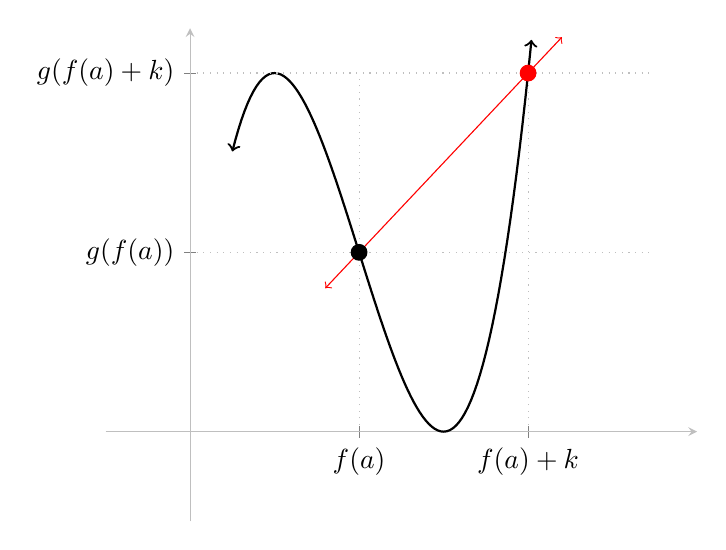
\begin{tikzpicture}
			\begin{axis}[
			xmin=-0.5,xmax=3,
			ymin=-0.5,ymax=2.25,
			ytick={1, 2},
			xtick={1,2},
			xticklabels={$f(a)$, $f(a)+k$},
			yticklabels={$g(f(a))$,$g(f(a)+k)$},
			axis lines=middle,
			axis line style=lightgray,
			width=0.75\textwidth
			]
			\addplot[black,style=thick,<->] expression[domain=0.25:2.02,samples=100]{4*x^3-12*x^2+9*x}; 
			
			
			\addplot[red,<->] expression[domain=0.8:2.2,samples=2]{(x-1)+1}; 
			
			
			\addplot[lightgray,dotted] expression[domain=0:2.75,samples=2]{1};
			\addplot[lightgray,dotted] expression[domain=0:2.75,samples=2]{2}; 
			\addplot +[mark=none,lightgray,dotted] coordinates {(1, 0) (1, 2)};
			\addplot +[mark=none,lightgray,dotted] coordinates {(2, 0) (2, 2)};
			
			\node[color=black,draw=black,circle,fill,inner sep=2pt] at (axis cs:1,1) {}; 
			
			\node[color=red,draw=red,circle,fill,inner sep=2pt] at (axis cs:2,2) {}; 
			\end{axis}
			\end{tikzpicture}
		\end{center}
		\caption{The graph of $g$ is depicted in black. The output of the function $\sigma$ on a small nonzero input value $k$ is the slope of the red secant line passing through the two points $(f(a), g(f(a))$ and $(f(a)+k, g(f(a)+k))$. }  \label{slope-function-chain-rule}
	\end{figure}
	
	
	You will verify in \cref{chain-rule-single-first-proof-details} below that
	\begin{equation} \label{alternative-to-multiplicative-cross-term} \frac{(g \circ f)(a+h) - (g \circ f)(a)}{h} = \sigma(\Delta(h)) \cdot \frac{f(a+h)-f(a)}{h} \end{equation}
	for all small values of $h$. Thus
	\[ \lim_{h \to 0} \frac{(g \circ f)(a+h) - (g \circ f)(a)}{h} = \lim_{h \to 0} \sigma (\epsilon(h)) \cdot \frac{f(a+h)-f(a)}{h} = g'(f(a)) f'(a) \]
	where we have used the continuity of $\epsilon$ and $\sigma$ and the definition of the derivative of $f$ at $a$ for the last step. This completes the proof. 
\end{proof}
	
\begin{exercise} \label{chain-rule-single-first-proof-details}
	Prove \cref{alternative-to-multiplicative-cross-term}. 
	\begin{hint} You might split up your proof of \cref{alternative-to-multiplicative-cross-term} into two cases: when $f(a+h) \neq f(a)$, and when $f(a+h) = f(a)$. 
	\end{hint}
\end{exercise}

\subsubsection*{Second proof}

Our second proof of the chain rule will use the ``best linear approximation'' interpretation of derivatives provided by \cref{differential-unique-single}. 

\begin{proof}[Second proof of the chain rule] \renewcommand{\qedsymbol}{}
	Note that, by definition of $dg_{f(a)}$ and $df_a$, we have 
	\[ dg_{f(a)}(df_a(h)) = g'(f(a))f'(a)h. \]
	Thus, by \cref{differential-unique-single}, it is sufficient to prove that
	\[ g(f(a+h))-g(f(a))-dg_{f(a)}(df_a(h)) = o(|h|) \text{ as } h \to 0. \]
	In other words, we want to prove that $g(f(a+h))-g(f(a))-dg_{f(a)}(df_a(h))$ is ``small.'' What we know is that the following remainder functions are ``small'' (cf. \cref{remainder-linear}).
	\[ \begin{aligned} 
	r(h) &= f(a+h)-f(a) - df_a(h) \\ 
	s(k) &= g(f(a)+k)-g(f(a))-dg_{f(a)}(k) \end{aligned} \]
	So the gist of the proof is to rewrite $g(f(a+h))-g(f(a))-dg_{f(a)}(df_a(h))$ in terms of $r$ and $s$, and then prove that it is ``small'' using the facts that $r$ and $s$ are ``small.''
	
	Rearranging the definition of $r(h)$ tells us that
	\begin{equation} \label{rearranged-definition-error} g(f(a+h)) = g(f(a) + df_a(h) + r(h)). \end{equation}
	Now note that the definition of $s(k)$ for $k = df_a(h) + r(h)$ says the following. 
	\[ \begin{aligned} s(df_a(h) + r(h)) &= g(f(a) + df_a(h) + r(h)) - g(f(a)) -dg_{f(a)}(df_a(h) + r(h)) \\
	g(f(a) + df_a(h) + r(h)) &= g(f(a)) + dg_{f(a)}(df_a(h) + r(h)) + s(df_a(h) + r(h)) \\
	&= g(f(a)) + dg_{f(a)}(df_a(h)) + dg_{f(a)}(r(h)) + s(df_a(h) + r(h))  \end{aligned} \]
	We used linearity of $dg_{f(a)}$ for the final step above. Combining this with \cref{rearranged-definition-error} show that
	\[ g(f(a+h)) - g(f(a)) - dg_{f(a)}(df_a(h)) = dg_{f(a)}(r(h)) + s(df_a(h)+r(h)). \]
	At this point, we've rewritten $g(f(a+h))-g(f(a))-dg_{f(a)}(df_a(h))$ in terms of $r$ and $s$. We'll now prove that the right-hand side is in fact ``small'', ie, that it is $o(|h|)$. Observe that \[ dg_{f(a)}(r(h)) = g'(f(a)) \cdot r(h), \] ie, $dg_{f(a)} \circ r$ is just a scalar multiple of $r$. We know that $r(h) = o(|h|)$ as $h \to 0$, so it follows that $dg_{f(a)}(r(h)) = o(|h|)$ also. So it is sufficient to prove that
	\[ s(df_a(h)+r(h)) = o(|h|). \]
	We've now hit the technical part, so let's hit pause. 
\end{proof}

To see why this is technical, and for essentially the same reasons as the previous proof, notice that we're trying to prove that
\[ \lim_{h \to 0} \frac{|s(df_a(h)+r(h)|)}{|h|} = 0.  \]
To prove this, it's tempting to introduce a multiplicative cross-term as follows. 
\[ \frac{|s(df_a(h)+r(h)|)}{|h|} = \frac{|s(df_a(h)+r(h)|)}{|df_a(h)+r(h)|} \cdot \frac{|df_a(h)+r(h)|}{|h|} \]
But notice that $df_a(h)+r(h) = f(a+h)-f(a)$ by definition of $r$, so this cross term is problematic for the same reasons as before! If $f(a+h) = f(a)$ for $h$ arbitrarily close to $0$, we have an infinite sequence of divisions by zeroes that causes problems. 

We'll deal with this problem in essentially the same way as before: namely, we extend the definition of 
\[\frac{|s(df_a(h)+r(h)|)}{|df_a(h)+r(h)|}\]
so that it is also defined when $f(a+h) = f(a)$. 

\begin{proof}[Second proof of the chain rule, continued]
	Define $\eta(k) = s(k)/k$ for nonzero $k$. Then extend $\eta$ by setting $\eta(0) = 0$. The fact that $s(k) = o(|k|)$ as $k \to 0$ implies that $\eta$ is continuous at 0. We now have \[ s(k) = \eta(k)k \]
	for all $k$. Applying this with $k = df_a(h) + r(h)$, we see that
	\[ \begin{aligned} \frac{|s(df_a(h)+r(h))|}{|h|} &= \frac{|\eta(df_a(h)+r(h))| \cdot |df_a(h)+r(h)|}{|h|} \\
	&\leq |\eta(df_a(h)+r(h))| \cdot \left( |f'(a)| + \frac{|r(h)|}{|h|} \right). \end{aligned} \]
	Since $r$ is continuous at 0 (cf. \cref{remainder-linear}), so is $df_a + r$. We have $(df_a + r)(0) = 0$, and we have just seen that $\eta$ is also continuous at $0$. Thus the composite $\eta \circ (df_a + r)$ is continuous at 0. Thus
	\[ \lim_{h \to 0} |\eta(df_a(h)+r(h))| \cdot \left( |f'(a)| + \frac{|r(h)|}{|h|} \right) = 0, \]
	where we have used the fact that $|r(h)| = o(|h|)$ to see that the parenthetical expression has a finite limit (namely, $|f'(a)|$). So, by the squeeze theorem, we can conclude that \[ |s(df_a(h)+r(h))| = o(|h|). \qedhere \]   
\end{proof}

Notice that in the first proof, the trick to overcoming the technicality was defining the function $\sigma$ at $k = 0$. In the second proof, the trick to overcoming the same technicality was defining $\eta$ at $k = 0$. These two tricks are really the same trick, as shown by the following.  

\begin{exercise}
	Prove that the function $\eta$ from the second proof and the function $\sigma$ from the first proof are related by the equation
	\[ \sigma(k) = g'(f(a)) + \eta(k). \]
\end{exercise}

\subsection{Interior extremum theorem}

We first recall the following definitions. 

\begin{definition} \index{extremum!local extremum} \index{extremum!local maximum} \index{extremum!local minimum} \index{extremum!absolute maximum} \index{extremum!absolute minimum} \index{extremum!absolute extremum}
	Supppose $X$ is a set, $f : X \to \R$ is a function, and $a \in X$. 
	\begin{itemize}
		\item $a$ is an \emph{absolute maximum}, or just \emph{maximum}, of $f$ if $f(x) \leq f(a)$ for all $x \in X$. 
		\item $a$ is a \emph{strict absolute maximum}, or just \emph{strict maximum} of $f$ if $f(x) < f(a)$ for all $x \in X \setminus\{a\}$. 
		\item $a$ is an \emph{absolute minimum}, or just \emph{minimum}, of $f$ if $f(x) \geq f(a)$ for all $x \in X$. 
		\item $a$ is a \emph{strict absolute minimum}, or just \emph{strict minimum} of $f$ if $f(x) > f(a)$ for all $x \in X \setminus\{a\}$. 
		\item $a$ is a \emph{absolute extremum}, or just \emph{extremum}, if it is either an absolute maximum or an absolute minimum. Similarly, $a$ is a \emph{strict absolute extremum}, or just \emph{strict extremum}, if it is either a strict absolute maximum or a strict absolute minimum. 
	\end{itemize}
	If $X$ is a metric space\footnotemark, we can also make the following definitions. 
	\begin{itemize}
		\item $a$ is a \emph{local maximum} of $f$ if there exists a neighborhood $U$ of $a$ in $X$ such that $f(x) \leq f(a)$ for all $x \in U$. 
		\item $a$ is a \emph{strict local maximum}, or just \emph{strict maximum} of $f$ if there exists a neighborhood $U$ of $a$ in $X$ such that $f(x) < f(a)$ for all $x \in U \setminus\{a\}$. 
		\item $a$ is a \emph{local minimum} of $f$ if there exists a neighborhood $U$ of $a$ in $X$ such that $f(x) \geq f(a)$ for all $x \in U$. 
		\item $a$ is a \emph{strict local minimum}, or just \emph{strict minimum} of $f$ if there exists a neighborhood $U$ of $a$ in $X$ such that $f(x) > f(a)$ for all $x \in U \setminus\{a\}$.
		\item $a$ is a \emph{local extremum} if it is either a local maximum or a local minimum. Similarly, $a$ is a \emph{strict local extremum} if it is either a strict local maximum or a strict local minimum. 
	\end{itemize}
\end{definition}

\footnotetext{For the definition of local extremums, $X$ could also be a topological space.}

The following is a key property of derivatives that you probably remember using frequently when you were first exposed to calculus. 

\begin{exercise}[Interior extremum theorem] \label{interior-extremum} \index{extremum!interior extremum theorem} \index{interior extremum theorem|see {extremum}}
	Suppose an interior point $a \in S$ is a local extremum of a function $f : S \to \R$. If $f$ is differentiable at $a$, prove that $f'(a) = 0$.
	\begin{hint} 
		Consider the following ``slope of secant'' function (which we've seen before, during the first proof of the chain rule in \cref{chain-rule-single-section}).
		\[ \sigma(h) = \begin{cases} \dfrac{f(a+h)-f(a)}{h} & \text{if } h \neq 0 \\ f'(a) & \text{if } h = 0 \end{cases} \]
		Since $f$ is differentiable at $x = a$, we know that $\sigma$ is continuous at $h = 0$. If $a$ is a local minimum, what can you say about the values of $\sigma$ for positive values of $h$? Negative values of $h$? Then consider the case when $a$ is a local maximum. 
	\end{hint}
\end{exercise}

But remember, the converse to the interior extremum theorem \ref{interior-extremum} is \emph{not} true. 

\begin{exercise} \label{interior-extremum-converse-false}
	Give an example of a function $f : \R \to \R$ such that $f'(0) = 0$, but $f$ does not have a local extremum at 0.\index{extremum!local extremum} 
\end{exercise}

\subsection{Non-rational functions} \label{non-rational}

Using the rules we've developed so far, we can differentiate any rational function (ie, a quotient of a polynomial by a polynomial). In this section, we will simply state some facts about differentiation of other types of functions one frequently encounters. We will prove most of these a bit later; we are stating them now so that we can discuss a richer repertoire of examples as we go along. We've already seen the need for a richer repertoire of examples in \cref{wrong-conjecture-counterexample}. 

\subsubsection*{Power rule}

First off, here is the most general statement of the power rule.

\begin{proposition}[Power rule for real exponents] \label{power-rule-general} \index{power rule}
	If $r$ is any real number and $f : (0, \infty) \to \R$ is the function $f(x) = x^r$, then $f'(x) = rx^{r-1}$ for all $x \in (0,\infty)$. 
\end{proposition}

We'll prove this for \emph{rational} exponents (ie, exponents that can be written as fractions of an integer over another integer) in \cref{power-rule-fractional}. We won't prove it in full generality, because that would require a long tangential discussion of what $x^r$ even means for irrational $r$. Actually, once we have a sufficiently rigorous definition of $x^r$ for irrational $r$, it turns out that \cref{power-rule-general} is actually a relatively straightforward \emph{consequence} of \cref{power-rule-fractional}. 

\subsubsection*{Exponential, sine, and cosine functions}

Next up, we have the exponential, sine, and cosine functions. These are usually defined by their power series\index{power series}, as follows. 
\begin{equation} \label{exp-sin-cos-power-series} \begin{aligned} \exp(x) &= \sum_{n = 0}^\infty \frac{x^n}{n!} \\
\cos(x) &= \sum_{n = 0}^\infty \frac{(-1)^n x^{2n}}{(2n)!} \\
\sin(x) &= \sum_{n = 0}^\infty \frac{(-1)^n x^{2n+1}}{(2n+1)!} \end{aligned} \end{equation}
All three of these have infinite radius of convergence (ie, they're defined for all real $x$). We'll prove that power series can be differentiated term-by-term in \cref{differentiating-power-series} inside their radius of convergences. This yields the following standard facts. 
\begin{enumerate}[(1)]
	\item If $f(x) = \exp(x)$, then $f'(x) = \exp(x)$. 
	\item If $f(x) = \sin(x)$, then $f'(x) = \cos(x)$. 
	\item If $f(x) = \cos(x)$, then $f'(x) = -\sin(x)$.
\end{enumerate} 

\begin{pedanticremark}
	Defining the exponential, sine, and cosine functions using power series is mathematically sound, but there are numerous facts about these functions that are not clear from the power series. For example, it's useful knowing that, if $e := \exp(1)$, then $\exp(x) = e^x$. This fact is not immediately clear from the power series definition; it requires some proof, and we won't prove it here, but you should feel free to use it. It's obviously also useful to know that sines and cosines have something to do with trigonometry. Again, this is not clear from the power series definition; it requires some proof, and we won't prove it, but you should feel free to use it. 
\end{pedanticremark}

% TODO: Geometric proof of the derivative of sines and cosines

\subsubsection*{Examples}

Let's now discuss some examples using these functions. The following two examples both involve the expression $\sin(1/x)$. As we will see, functions involving this expression exhibit a wild variety of interesting pathological behavior. 

\begin{exercise} \label{power-times-sine}
	\begin{enumerate}[(a)]
		\item Prove that the function \[ f(x) = \begin{cases} \sin(1/x) & \text{if } x \neq 0 \\ 0 & \text{if } x = 0 \end{cases} \]
		is discontinuous at 0. 
		
		\begin{hint}
			Show the following. 
			\[ \limsup_{x \to 0^{\pm}} \sin(1/x) = 1 \quad\quad \liminf_{x \to 0^{\pm}} \sin(1/x) = -1 \]
		\end{hint}
	
		\item Prove that the function \[ f(x) = \begin{cases} x\sin(1/x) & \text{if } x \neq 0 \\ 0 & \text{if } x = 0 \end{cases} \]
		is continuous, but that it is not differentiable at 0. 
		\item Prove that the function \[ f(x) = \begin{cases} x^2\sin(1/x) & \text{if } x \neq 0 \\ 0 & \text{if } x = 0 \end{cases} \]
		is differentiable, but that the derivative $f'$ is not continuous at 0.  
	\end{enumerate} 
\end{exercise}

The following example, again involving $\sin(1/x)$, illustrates a caveat to the interior extremum theorem \cref{interior-extremum}: even if $f$ has a local extremum at a point, it need not be that the derivative ``changes sign'' at that point.

\begin{exercise} \label{extremum-no-sign-change}
	Consider the function $f : \R \to \R$ given by 
	\[ f(x) = \begin{cases} x^4 \left( 2 + \sin(1/x) \right) & \text{if } x \neq 0 \\ 0 & \text{if } x = 0. \end{cases} \]
	\begin{enumerate}[(a)]
		\item Show that $f$ has an absolute minimum at 0.\index{extremum!absolute minimum} 
		\item Show that $f$ is differentiable and calculate the derivative $f'$. 
		\item Show that, on every open interval of the form $(a, 0)$ or $(0, b)$, the derivative $f'$ takes on both positive and negative values. 
	\end{enumerate}
\end{exercise}

\section{Differentiable functions} \label{single-differentiable}

In this section, we'll discuss some properties of functions which are differentiable everywhere on their domain. 

\begin{definition} \label{differentiable-open-domain-single} \index{differentiable} \index{derivative}
	Suppose $U$ is an open subset of $\R$. A function $f : U \to \R$ is \emph{differentiable} if it is differentiable at every point in $U$. The function $U \to \R$ given by $x \mapsto f'(x)$ is called the \emph{derivative} of $f$, and is denoted $f'$. 
\end{definition}

Every open subset of $\R$ is a countable disjoint union of open intervals\footnotemark\ (cf. \cite[theorem 6.17]{protter-morrey}), so the most important case of the above definition is when the domain happens to be an open interval. Occasionally, it's also useful to have some vocabulary for talking about functions on non-open intervals. Here is the ``correct'' definition for doing this.

\footnotetext{By the word \emph{interval}\index{interval}, we mean an uncountable connected subset of $\R$. This means that intervals can be open, closed, or half-open; and they can be bounded or unbounded. They cannot be just a single point.}

\begin{definition} \label{differentiable-any-domain-single}
	Suppose $S$ is any subset of $\R$ and $f : S \to \R$ is a function.
	\begin{itemize}
		\item We say that $f$ is \emph{differentiable on the interior} if $f$ is differentiable at every interior point of $S$ (ie, if the restriction of $f$ to the interior $S^\circ$ is differentiable in the sense of \cref{differentiable-open-domain-single}). The function $S^\circ \to \R$ given by $x \mapsto f'(x)$ is called the \emph{derivative} of $f$, and is denoted $f'$. 
		\item We say that $f$ is \emph{differentiable} if it is the restriction to $S$ of a differentiable function defined on an open neighborhood of $S$.  The function $S \to \R$ given by $x \mapsto f'(x)$ is called the \emph{derivative} of $f$, and is denoted $f'$. 
	\end{itemize} 
\end{definition}

\begin{pedanticremark}
	The reason these definitions are made the way they are is for precisely the same reasons discussed in the pedantic remark towards the end of \cref{slope-of-tangent-line}. 
\end{pedanticremark}

\subsection{Mean value theorem}

The mean value theorem \ref{mean-value-theorem}\index{mean value theorem} is an extremely important foundational result. You may remember seeing and ignoring it during your first calculus class; at least, that's what I did, and I think that's okay. Its importance largely derives from the fact that it comes up incredibly frequently when proving things formally about derivatives. 

\begin{theorem}[Mean value theorem]  \label{mean-value-theorem}
	Suppose $a < b$ and let $f : [a, b] \to \R$ be continuous and differentiable on the interior. Then there exists $c \in (a, b)$ such that
	\[ f'(c) = \frac{f(b) - f(a)}{b-a}. \]
\end{theorem}

Before proceeding, I encourage you to look at \cref{mean-value-theorem-picture} and ensure that you understand the geometric content of the statement. 

\begin{figure}
	\begin{center}
	\begin{tikzpicture}
	\begin{axis}[
	xmin=-0.1,xmax=2.5,
	ymin=-0.1,ymax=2,
	ytick={0.5, 1.5},
	xtick={0.5, 0.892375, 2},
	xticklabels={$a$, $c$, $b$},
	yticklabels={$f(a)$, $f(b)$},
	axis lines=middle,
	axis line style=lightgray,
	width=\textwidth
	]
	\addplot[black,thick,-] expression[domain=0.5:2,samples=50]{2/3*x+1/6 + 2*(x-0.5)*(x-1.5)*(x-2)}; 
	
	
	\addplot[black,<->] expression[domain=0.25:2.25,samples=2]{2/3*x+1/6}; 
	\addplot[red,<->] expression[domain=0.25:1.75,samples=2]{2/3*x+0.694821}; 
	
	
	\addplot[lightgray,dotted] expression[domain=0:2.75,samples=2]{0.5};
	\addplot[lightgray,dotted] expression[domain=0:2.75,samples=2]{1.5}; 
	\addplot +[mark=none,lightgray,dotted] coordinates {(0.5, 0) (0.5, 2)};
	\addplot +[mark=none,lightgray,dotted] coordinates {(2, 0) (2, 2)};
	
	
	\node[color=red,draw=red,circle,fill,inner sep=2pt] at (axis cs:0.892375,1.28974) {};
	\node[color=black,draw=black,circle,fill,inner sep=2pt] at (axis cs:0.5,0.5) {}; 
	\node[color=black,draw=black,circle,fill,inner sep=2pt] at (axis cs:2,1.5) {}; 
	\end{axis}
	\end{tikzpicture}
	\end{center}

	\caption{The mean value theorem \ref{mean-value-theorem} states that, if we draw a secant line connecting two points $(a,f(a))$ and $(b,f(b))$ on the graph of a differentiable function $f$, then that secant line must be parallel to the tangent line of $f$ at some point $c$ in between $a$ and $b$. The statement of the mean value theorem only asserts existence, not uniqueness; there could be multiple points $c$ at which this happens.} \label{mean-value-theorem-picture} 
\end{figure}

\begin{caution}
	Despite the similar sounding name, the mean value theorem is \emph{not} the same as the intermediate value theorem! The intermediate value theorem asserts that, if $f : [a,b] \to \R$ is continuous and $y$ is in between $f(a)$ and $f(b)$, then there exists $c \in (a,b)$ such that $f(c) = y$. The output of the intermediate value theorem is a point $c$ where the value of the function itself is some desired value (specifically, some value between $f(a)$ and $f(b)$), while the output of the mean value theorem is a point $c$ where the value of the \emph{derivative} is some desired value (specifically, the slope of the secant connecting $((a,f(a))$ and $(b,f(b))$. 
\end{caution}

Rolle's theorem \ref{rolles-theorem} is technically a special case of the mean value theorem, but the general case can be derived from this special case. 

\begin{exercise}[Rolle's theorem] \label{rolles-theorem} \index{mean value theorem!rolles theorem@Rolle's theorem} \index{rolles theorem@Rolle's theorem|see {mean value theorem}}
	Suppose $a < b$ and let $f : [a, b] \to \R$ be continuous and differentiable on the interior. If $f(a) = f(b) = 0$, prove that there exists $c \in (a, b)$ such that $f'(c) = 0$. 
	\begin{hint}
		Notice that any function must fall into at least one of the following three cases: (i) $f$ is constantly zero, (ii) $f$ takes on positive values somewhere on $[a, b]$, and (iii) $f$ takes on negative values somewhere on $[a, b]$. Deal with the first case using \cref{constant-implies-derivative-zero-single}, and the latter two cases using the extreme value theorem\footnotemark\ together with the interior extremum theorem \cref{interior-extremum}. 
	\end{hint}
\end{exercise}

\footnotetext{The \emph{extreme value theorem}\index{extremum!extreme value theorem} \index{extreme value theorem|see {extremum}} says that if $K$ is a compact metric space and $f : K \to \R$ is continuous, then $f$ achieves its global maximum and its global minimum somewhere on $K$ (cf. \cite[theorems 3.17 and 6.30]{protter-morrey}).}

\begin{exercise}
	Prove the mean value theorem. 
	\begin{hint} 
		Let $\ell$ be the secant line passing through $(a, f(a))$ and $(b, f(b))$. Then consider the function $g = f - \ell$. See \cref{subtracting-the-secant}. 
		Then $g(a) = g(b) = 0$, so we can apply Rolle's theorem \ref{rolles-theorem} to $g$.
	\end{hint} 
\end{exercise}

\begin{figure}
	\begin{center}
		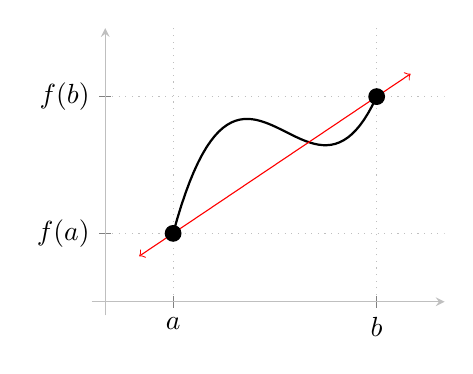
\begin{tikzpicture}
		\begin{axis}[
		xmin=-0.1,xmax=2.5,
		ymin=-0.1,ymax=2,
		ytick={0.5, 1.5},
		xtick={0.5,2},
		xticklabels={$a$, $b$},
		yticklabels={$f(a)$, $f(b)$},
		axis lines=middle,
		axis line style=lightgray,
		width=0.5\textwidth
		]
		\addplot[black,thick,-] expression[domain=0.5:2,samples=50]{2/3*x+1/6 + 2*(x-0.5)*(x-1.5)*(x-2)}; 
		
		
		\addplot[red,<->] expression[domain=0.25:2.25,samples=2]{2/3*x+1/6}; 
		
		
		\addplot[lightgray,dotted] expression[domain=0:2.75,samples=2]{0.5};
		\addplot[lightgray,dotted] expression[domain=0:2.75,samples=2]{1.5}; 
		\addplot +[mark=none,lightgray,dotted] coordinates {(0.5, 0) (0.5, 2)};
		\addplot +[mark=none,lightgray,dotted] coordinates {(2, 0) (2, 2)};
		
		
		\node[color=black,draw=black,circle,fill,inner sep=2pt] at (axis cs:0.5,0.5) {}; 
		\node[color=black,draw=black,circle,fill,inner sep=2pt] at (axis cs:2,1.5) {}; 
		\end{axis}
		\end{tikzpicture}\hspace{1cm}
		\begin{tikzpicture}
		\begin{axis}[
		xmin=-0.1,xmax=2.5,
		ymin=-1,ymax=1.1,
		ytick={0},
		xtick={0.5,2},
		xticklabels={$a$, $b$},
		yticklabels={},
		axis lines=middle,
		axis line style=lightgray,
		width=0.5\textwidth
		]
		\addplot[black,thick,-] expression[domain=0.5:2,samples=50]{2*(x-0.5)*(x-1.5)*(x-2)}; 
		
		\addplot[red,<->] expression[domain=0.25:2.25,samples=2]{0};
		
		\addplot +[mark=none,lightgray,dotted] coordinates {(0.5, -2) (0.5, 2)};
		\addplot +[mark=none,lightgray,dotted] coordinates {(2, -2) (2, 2)};
		
		\node[color=black,draw=black,circle,fill,inner sep=2pt] at (axis cs:0.5,0) {}; 
		\node[color=black,draw=black,circle,fill,inner sep=2pt] at (axis cs:2,0) {}; 
		\end{axis}
		\end{tikzpicture}
	\end{center}
	\caption{On the left is depicted the graph of a function $f$ and the secant line $\ell$. Subtracting $\ell$ from the picture on the left yields the picture on the right. }  \label{subtracting-the-secant}
\end{figure}

We can use the mean value theorem to prove the following ``if and only if upgrade'' of \cref{constant-implies-derivative-zero-single}. 

\begin{proposition} \label{constant-iff-derivative-zero-single}
	Suppose $I$ is an interval and that $f : I \to \R$ is continuous and differentiable on the interior. Then $f' = 0$ if and only if $f$ is constant\index{constant function}. 
\end{proposition}

\begin{proof}
	We showed in \cref{constant-implies-derivative-zero-single} that $f$ being constant implies $f' = 0$. Conversely, suppose we have $a < b$ in $I$. We want to show that $f(a) = f(b)$. Since $f$ is continuous and differentiable on the interior, the same is true on the compact subinterval $[a,b]$, so we can apply the mean value theorem on this interval. In other words, there exists a point $c \in (a,b)$ such that
	\[ \frac{f(b)-f(a)}{b-a} = f'(c). \]
	But $f'(c) = 0$ by assumption, so $f(a) = f(b)$. 
\end{proof}

Here are some more consequences. 

\begin{exercise} \label{bounded-derivative}
	Suppose $I$ is an interval and $f : I \to \R$ is continuous and differentiable on the interior. Let $M$ be a real number. Show that $|f'(x)| \leq M$ if and only if for all $x \in I$ if and only if \[ |f(b) - f(a)| \leq M|b-a| \] for all $a, b \in I$.
\end{exercise}

\begin{unimportantremark}
	Another way of stating the result of \cref{bounded-derivative} is that bounds on the derivative of $f$ are equivalent to \emph{Lipschitz constants} for $f$. In particular, having a bounded derivative implies \emph{Lipschitz continuity}. 
\end{unimportantremark}

\begin{exercise}[Fixed points] \label{fixed-points}
	Suppose $f : \R \to \R$ is a function. A \emph{fixed point} of $f$ is a point $\xi$ such that $f(\xi) = \xi$. 
	\begin{enumerate}[(a)]
		\item Suppose $f$ is differentiable and $f'(x) \neq 1$ for all $x \in \R$. Prove that $f$ has at most one fixed point. 
		\item Suppose $f$ is differentiable and there exists a constant $M < 1$ such that $|f'(x)| \leq M$ for all $x \in \R$.\footnote{Using the vocabulary of \cref{sup-norm}, this hypothesis can be rephrased by saying that $\|f'\|_\spn < 1$.}\ Show that $f$ has a unique fixed point.  
		
		\begin{hint}
			Pick any $x_0 \in \R$, and then inductively define $x_{n+1} = f(x_n)$ for all $n$. Prove inductively that $|x_{n+1} - x_n| \leq M^n|x_1 - x_0|$ for all $n$. Deduce that the sequence $x_0, x_1, x_2, \dotsc$ is Cauchy, and let $\xi = \lim x_n$. Then show that $\xi$ is a fixed point of $f$. 
		\end{hint}
	
		\item Suppose $f(x) = x + 1/(1 + \exp(x))$.
		Show that $f$ has no fixed points, and that $f$ is differentiable with $0 < f'(x) < 1$ for all $x \in \R$. Explain why this does not contradict part (b). 
	\end{enumerate}
\end{exercise}

\begin{exercise}[``Leveling off'' vs ``flattening out''] \label{leveling-off-vs-flattening-out}
	\begin{enumerate}[(a)]
		\item Suppose $f : (0, \infty) \to \R$ is differentiable and $f(x) \to 0$ as $x \to \infty$ (one might say informally that $f$ ``levels off'' near infinity). Show that, if 
		\[ \lim_{x \to \infty} f'(x) \]
		exists, then this limit must equal 0 (informally, one might say that that $f$ must ``flatten out'' near infinity).
		\item Let $f : (0, \infty) \to \R$ be defined by 
		\[ f(x) = \frac{\sin(x^2)}{x}. \]
		Show that ``levels off'' but does not ``flatten out'' near infinity.  
	\end{enumerate}
\end{exercise}

\begin{exercise}
	Suppose $f : \R \to \R$ is differentiable which ``flattens out'' near infinity; in other words, \[ \lim_{x \to \infty} f'(x) = 0. \] Let $g(x) = f(x+1) - f(x)$. Is it true that $g$ ``levels off'' near infinity (ie, that $g(x) \to 0$ as $x \to \infty$)? If so, prove it. If not, explain why not. 
\end{exercise}

\begin{exercise} \label{continuous-and-differentiable-except-at-point}
	Let $I$ be an open interval and $a \in I$. Suppose that $f : I \to \R$ is continuous, and suppose further that it is differentiable at every $x \in I$ except possibly at $a$. If \[ \lim_{x \to a} f'(x) \]
	exists, show that $f$ is also differentiable at $a$ and that $f'(a)$ is equal to this limit. 
\end{exercise}

\subsection{Monotonicity}

We begin by recalling the following definition. 

\begin{definition} \index{monotone} \index{monotone!increasing} \index{monotone!decreasing} \index{monotone!strictly monotone} \index{monotone!strictly increasing} \index{monotone!strictly decreasing} 
	Suppose $I$ is an interval and $f : I \to \R$ is a function.
	\begin{itemize}
		\item $f$ is \emph{increasing} $f(x) \leq f(y)$ for all $x < y$ in $I$. 
		\item $f$ is \emph{decreasing} $f(x) \geq f(y)$ for all $x < y$ in $I$.
		\item $f$ is \emph{strictly increasing} $f(x) < f(y)$ for all $x < y$ in $I$. 
		\item $f$ is \emph{strictly decreasing} $f(x) > f(y)$ for all $x < y$ in $I$. 
	\end{itemize}
Further, $f$ is \emph{monotone} if it is either increasing or decreasing, and \emph{strictly monotone} if it is either strictly increasing or strictly decreasing. 
\end{definition}

Here are some important properties of strictly monotone continuous functions.

\begin{exercise} \label{strictly-monotone-iff-injective}
	Suppose $I$ is an interval and $f : I \to \R$ is continuous. Prove that $f$ is injective if and only if $f$ is strictly monotone. 
\end{exercise}

\begin{exercise} \label{strictly-monotone-implies-open}
	Prove that, if $I$ is an open interval and $f : I \to \R$ is continuous and strictly monotone, then $f(I)$ is also an open interval. Conclude that $f$ is an open map\index{open!open map} (ie, that the image of any open subset of the domain is an open subset of $\R$).
	\begin{hint}
		Suppose $f$ is strictly increasing and $I = (a, b)$. Define $c = \lim_{x \to a^+} f(x)$ and $d = \lim_{x \to b^-} f(x)$ and use the intermediate value theorem to prove that $f(I) = (c, d)$. Then deal with the case when $f$ is strictly decreasing. 
	\end{hint}
\end{exercise}

The proofs of the following standard relationships between derivatives and monotonicity are similar to the proof of \cref{constant-iff-derivative-zero-single}.

\begin{exercise}[Derivatives and monotonicity] \label{monotone-derivative}
	Suppose $I$ is an interval and that $f : I \to \R$ is continuous and differentiable on the interior. 
	\begin{enumerate}[(a)]
		\item Prove that $f' \geq 0$ if and only if $f$ is increasing. 
		\item Prove that $f' \leq 0$ if and only if $f$ is decreasing.
	\end{enumerate}
	\begin{hint}
		You could basically repeat your proof of part (a) for part (b). Alternatively, notice that $f$ is decreasing if and only if $-f$ is increasing. 
	\end{hint}
\end{exercise}

\begin{solution}{\cref{monotone-derivative} part (a)}
	Suppose $f' \geq 0$ and $x < y$ in $I$. By the mean value theorem \ref{mean-value-theorem}, there exists $c$ between $x$ and $y$ such that 
	\[ \frac{f(y)-f(x)}{y-x} = f'(c) \geq 0. \]
	Since $y - x \geq 0$, this means that $f(y) \geq f(x)$, proving that $f$ is increasing. Conversely, suppose $f$ is increasing. Then for any $a \in I$ and $h > 0$, we have $f(a+h) \geq f(a)$, which means that 
	\[ \frac{f(a+h)-f(a)}{h} \geq 0 \]
	for all $h > 0$. Thus 
	\[ f'(a) = \lim_{h \to 0^+} \frac{f(a+h)-f(a)}{h} \geq 0, \]
	proving that $f' \geq 0$. 
\end{solution}

\begin{exercise}[Derivatives and strict monotonicity] \label{strictly-monotone-derivative}
	Suppose $I$ is an interval and that $f : I \to \R$ is continuous and differentiable on the interior. Prove the following. 
	\begin{enumerate}[(a)]
		\item If $f' > 0$, prove that $f$ is strictly increasing. 
		\item If $f' < 0$, prove that $f$ is strictly decreasing. 
		\item Unlike \cref{monotone-derivative}, the above two statements on strict monotonicity cannot be upgraded to ``if and only if'' statements. Give an example of a strictly increasing function $f : \R \to \R$ for which there exists some $a \in \R$ such that $f'(a) = 0$. 
		\item Notice that your proof of ``$f' \geq 0$ implies increasing'' from \cref{monotone-derivative} part (a) and ``$f' > 0$ implies strictly increasing'' from part (a) of this exercise are basically the same, except that all instances of ``$\geq$'' get replaced by ``$>$.'' Now inspect your proof of ``increasing implies $f' \geq 0$'' from \cref{monotone-derivative} part (a). Why can't you just replace all instances of ``$\geq$'' with ``$>$''?
	\end{enumerate} 
\end{exercise}

\begin{exercise}
	Suppose $f : \R \to \R$ is differentiable and there exists $M > 0$ such that $|f'(x)| \leq M$ for all $x \in \R$. Is it true that there must exist $\epsilon >  0$ such that the function $g : \R \to \R$ given by \[ g(x) = x + \epsilon f(x) \]
	is strictly increasing? If so, prove it. If not, explain why not. 
\end{exercise}

Again, there are pathologies involving monotonicity than can be exhibited by functions involving $\sin(1/x)$. Here is an example of a function whose derivative is positive at a single point, but it is not monotone near that point. 

\begin{exercise} \label{positive-not-monotone}
	Let $f : \R \to \R$ denote the function
	\[ f(x) = \begin{cases} x + 2x^2 \sin(1/x) & \text{if } x \neq 0 \\ 0 & \text{if } x = 0. \end{cases} \]
	\begin{enumerate}[(a)]
		\item Show that $f$ is differentiable and calculate $f'$. In particular, show that $f'(0) = 1$. 
		\item Show that $f$ is not monotone on any open interval containing 0.  
		\item Explain the ``2'' that shows up in the definition of $f$. Could it be replaced by 1 without changing the property of $f$ you proved in (b) above? Could it be replaced by 3? What is the set of all real numbers that it could be replaced with?
	\end{enumerate}
\end{exercise}

\subsection{Concavity}

Here is a word you probably recognize from calculus, but perhaps you haven't seen a formal definition. 

\begin{definition} \label{concave-up-definition}
	Suppose $I$ is an interval and $f : I \to \R$ is a function. We say that $f$ is \emph{concave up} (or \emph{convex}) if
	\[ \frac{f(y)-f(x)}{y-x} \leq \frac{f(z)-f(y)}{z-y} \]
	for all $x < y < z$ in $I$. 
	See \cref{concave-up-picture}. We say that $f$ is \emph{strictly concave up} (or \emph{strictly convex}) if 
	\[ \frac{f(y)-f(x)}{y-x} < \frac{f(z)-f(y)}{z-y} \]
	for all $x < y < z$ in $I$. 
	Similarly, we say that $f$ is \emph{concave down} (or just \emph{concave}) if
	\[ \frac{f(y)-f(x)}{y-x} \geq \frac{f(z)-f(y)}{z-y} \]
	for all $x < y < z$ in $I$, and we make an analogous definition for \emph{strictly concave down} (or just \emph{strictly concave}). 
\end{definition}

Notice that $f$ is (strictly) concave down if and only if $-f$ is (strictly) concave up. 

\begin{figure}[t]
	\begin{center}
		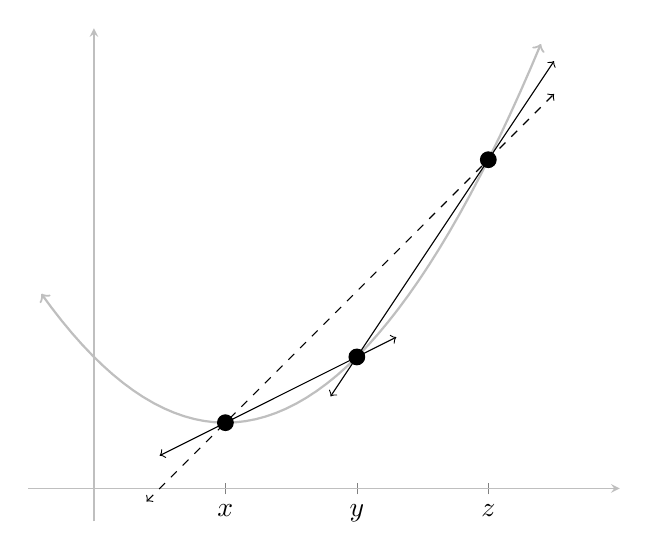
\begin{tikzpicture}
		\begin{axis}[
		xmin=-0.5,xmax=4,
		ymin=-0.5,ymax=7,
		xtick={1,2,3},
		ytick={0},
		xticklabels={$x$, $y$, $z$},
		yticklabels={},
		axis lines=middle,
		axis line style=lightgray,
		width=0.75\textwidth
		]
		\addplot[lightgray,style=thick,<->] expression[domain=-0.4:3.4,samples=50]{(x-1)^2+1}; 
		
		
		\addplot[black,<->] expression[domain=0.5:2.3,samples=2]{x}; 
		\addplot[black,<->] expression[domain=1.8:3.5,samples=2]{3*x-4};
		\addplot[black,dashed,<->] expression[domain=0.4:3.5,samples=2]{2*x-1};  
		
		\node[color=black,draw=black,circle,fill,inner sep=2pt] at (axis cs:1,1) {};
		\node[color=black,draw=black,circle,fill,inner sep=2pt] at (axis cs:2,2) {};
		\node[color=black,draw=black,circle,fill,inner sep=2pt] at (axis cs:3,5) {};
		
		\end{axis}
		\end{tikzpicture}
	\end{center}
	\caption{A function $f$ is defined to be \emph{concave up} in \cref{concave-up-definition} if the slope of the secant connecting $(x,f(x))$ and $(y,f(y))$ is less than or equal to the slope of the secant connecting $(y,f(y))$ and $(z,f(z))$ for all $x < y < z$. \Cref{concave-up-reformulation} says that, in this situation, the slope of the secant connecting $(x,f(x))$ and $(z,f(z))$ is in between the other two slopes. }  \label{concave-up-picture}
\end{figure}

\begin{lemma} \label{concave-up-reformulation}
	Suppose $I$ is an interval. A function $f : I \to \R$ is concave up if and only if 
	\[ \frac{f(y)-f(x)}{y-x} \leq \frac{f(z)-f(x)}{z-x} \leq \frac{f(z)-f(y)}{z-y} \]
	for all $x < y < z$ in $I$. 
\end{lemma}

\begin{proof}
	Clearly the double inequality in the statement of the lemma implies the single inequality in the definition. The proof of the converse is a rather unenlightening string of inequalities. 
	\begin{equation} \label{concave-up-reformulation-eqn1} \begin{aligned} \frac{f(y)-f(x)}{y-x} &\leq \frac{f(z)-f(y)}{z-y} \\
	(z-y)(f(y)-f(x)) &\leq (y-x)(f(z)-f(y)) \\
	zf(y) - zf(x) - yf(y) + yf(x) &\leq yf(z) - yf(y) - xf(z) +xf(y) \\
	zf(y) - zf(x) + yf(x) &\leq yf(z) - xf(z) + xf(y)
	\end{aligned} \end{equation}
	We'll take \cref{concave-up-reformulation-eqn1} and manipulate it to prove the two inequalities in the statement of the lemma. 
	
	First, if we take \cref{concave-up-reformulation-eqn1} and move the $yf(x)$ and $xf(y)$ terms to the opposite sides, and then add in $xf(x)$ to both sides, we see that 
	\[ \begin{aligned} 
	zf(y) - zf(x) - xf(y) &\leq yf(z) - yf(x) - xf(z) \\
	zf(y) - zf(x) - xf(y) + xf(x) &\leq yf(z) - yf(x) - xf(z) + xf(x) \\
	(z-x)(f(y)-f(x)) &\leq (y-x)(f(z)-f(x)) \\
	\frac{f(y)-f(x)}{y-x} &\leq \frac{f(z)-f(x)}{z-x},
	\end{aligned} \]
	which is one of the inequalities. On the other hand, if we move the $yf(z)$ and $zf(y)$ terms to the opposite sides in \cref{concave-up-reformulation-eqn1}, and then add in $zf(z)$ to both sides, we see that 
	\[ \begin{aligned} -zf(x) - yf(z) + yf(x) &\leq -zf(y) - xf(z) + xf(y) \\
	zf(z) -zf(x) - yf(z) + yf(x) &\leq zf(z) -zf(y) - xf(z) + xf(y) \\
	(z-y)(f(z)-f(x)) &\leq (z-x)(f(z)-f(y)) \\
	\frac{f(z)-f(x)}{z-x} &\leq \frac{f(z)-f(y)}{z-y}, \end{aligned} \]
	which is the other inequality. 
\end{proof}

\begin{unimportantremark}
	The proof above shows that either one of the two inequalities in the statement of \cref{concave-up-reformulation} implies that $f$ is concave up. 
\end{unimportantremark}

\begin{exercise}
	Suppose $f : [0, \infty) \to \R$ is concave up and that $f(0) = 0$. Show that the function $g : (0, \infty) \to \R$ defined by 
	\[ g(x) = \frac{f(x)}{x} \]
	is increasing. 
\end{exercise}

Here are some facts about how concavity relates to differentiation that you likely recognize from calculus. 

\begin{exercise}[Concavity and extremums] \label{concavity-extremums}
	Let $I$ be an open interval. Suppose $f : I \to \R$ is differentiable at a point $a \in I$ and $f'(a) = 0$. 
	\begin{enumerate}[(a)]
		\item If $f$ is concave up, show that $a$ is an absolute minimum of $f$. 
		\item If $f$ is concave down, show that $a$ is an absolute maximum of $f$. 
		\item If $f$ is strictly concave up, does it follow that $a$ is a strict absolute minimum of $f$? If so, prove it. If not, give a counterexample. 
	\end{enumerate} 
	\begin{hint}
		If $k < 0 < h$ and $f$ is concave up, then
		\[ \frac{f(a+k) - f(a)}{k} \leq \frac{f(a+h)-f(a)}{h}. \]
		Let $k \to 0^-$ to show that $a$ is a minimum on its right, and proceed similarly for the left. 
	\end{hint}
\end{exercise}

\begin{exercise}[Concavity and derivatives] \label{concavity-derivative}
	Suppose $I$ is an open interval and $f : I \to \R$ is differentiable. Prove the following. 
	\begin{enumerate}[(a)]
		\item $f$ is concave up if and only if $f'$ is increasing. 
		\item $f$ is concave down if and only if $f'$ is decreasing. 
		\item $f$ is strictly concave up if and only if $f'$ is strictly increasing. 
		\item $f$ is strictly concave down if and only if $f'$ is strictly decreasing. 
	\end{enumerate}
	\begin{hint}
		If $f'$ is (strictly) increasing, apply the mean value theorem \ref{mean-value-theorem} to prove that $f$ is (strictly) concave up. If $f$ is concave up, suppose we have $a < b$ in $I$. Let $x$ and $y$ be such that $a < x < y < b$. Explain why 
		\[ \frac{f(x)-f(a)}{x-a} \leq \frac{f(b)-f(y)}{b-y}, \]
		and then let $x \to a^+$ and $y \to b^-$. 
		The case when $f$ is \emph{strictly} concave up is a bit trickier (roughly because taking a limit can turn a $<$ into a  $\leq$), but one possible correct proof is a slight variant of the same idea. 
	\end{hint}
\end{exercise}

\subsection{Darboux's theorem \starred} \label{darboux-section}

Darboux's theorem asserts that derivatives are often ``close'' to being continuous, but in a weird way: they cannot have ``simple'' discontinuities, which means that when they are discontinuous at all, they are discontinuous in wild ways. 

\subsubsection*{Intermediate value property}

Before getting to the precise statement, we make the following definition. 

\begin{definition} \index{intermediate value property}
	Suppose $I$ is an interval and $f : I \to \R$ is a function. Then $f$ \emph{has the intermediate value property} if, for every $a < b$ in $I$ and every $y \in \R$ strictly between $f(a)$ and $f(b)$, there exists $x \in (a, b)$ such that $f(x) = y$.\footnote{Functions which have the intermediate value property are sometimes also called \emph{Darboux functions}.\index{Darboux function|see {intermediate value property}}} 
\end{definition}

Using this vocabulary, the intermediate value theorem\index{intermediate value theorem} asserts that every continuous function has the intermediate value property \cite[theorem 3.3]{protter-morrey}. Simple examples of discontinuous functions don't have the intermediate value property (cf. \cref{removable-jump-ivp} below). But, it turns out that some fairly bizarre discontinuous functions do have the intermediate value property (cf. \cref{discontinuous-ivp} below). 

\begin{exercise} \label{removable-jump-ivp}
	Let $I$ be an interval and $f : I \to \R$ a function. 
	\begin{enumerate}[(a)]
		\item Recall that $f$ has a \emph{removable discontinuity}\index{discontinuity!removable discontinuity} at a point $a \in I$ if
		\[ \lim_{x \to a} f(x) \]
		exists, but the value of this limit does not equal $f(a)$. Show that, if $f$ has a removable discontinuity, then $f$ does \emph{not} have the intermediate value property. 
		
		\item Recall that $f$ has a \emph{jump discontinuity}\index{discontinuity!jump discontinuity} at a point $a \in I$ if the two one-sided limits
		\[ \lim_{x \to a^-} f(x) \quad\text{ and }\quad \lim_{x \to a^+} f(x) \]
		both exist, but their values are not equal to each other. Show that, if $f$ has a jump discontinuity, then $f$ does \emph{not} have the intermediate value property.  
	\end{enumerate}
\end{exercise}

\begin{exercise} \label{discontinuous-ivp}
	Consider the function $f : \R \to \R$ defined by
	\[ f(x) = \begin{cases} \sin(1/x) & \text{if } x \neq 0 \\ 0 & \text{if } x = 0. \end{cases} \]
	We know from \cref{power-times-sine} that this function is discontinuous at 0. Show that it has the intermediate value property. \begin{hint} First show that for any interval $I$ containing 0, we have $f(I) = [-1,1]$. Then explain how this implies the intermediate value property. 
	\end{hint}
\end{exercise}

\subsubsection*{Statement of Darboux's theorem}

We know that the derivative $f'$ of a differentiable function $f$ need not be continuous (cf. \cref{power-times-sine}). Darboux's theorem asserts that, even though $f'$ might not be continuous, it must still have the intermediate value property! This means, for example, that derivatives cannot have removable or jump discontinuities (because, as we saw in \cref{removable-jump-ivp}, functions with these kinds of discontinuities do not have the intermediate value property). 

\begin{theorem}[Darboux] \label{darboux} \index{darbouxs theorem@Darboux's theorem}
	Suppose $I$ is an open interval and $f : I \to \R$ is differentiable. Then $f'$ has the intermediate value property.\index{intermediate value property} 
\end{theorem}

We noted earlier that the intermediate value theorem and the mean value theorem make similar but different assertions. Darboux's theorem now gets added to the fray! I encourage you to ensure that you understand how the statements of these three theorems differ (cf. \cref{ivt-mvt-darboux}).

\begin{table}
	\begin{center}
		{\scriptsize 
			\begin{tabular}{ p{0.17\textwidth} p{0.23\textwidth} p{0.23\textwidth} p{0.23\textwidth} } 
				\toprule[1pt]
				& Intermediate value theorem & Mean value theorem & Darboux's theorem \\ \cmidrule{2-4}
				If $f : [a, b] \to \R$ is... & continuous & continuous and differentiable on the interior & differentiable \\ \addlinespace[1em]
				& and $y$ is strictly in between $f(a)$ and $f(b)$ & & and $m$ is strictly in between $f'(a)$ and $f'(b)$ \\ \addlinespace[1em]
				then there exists $c$ in $(a,b)$ such that... & $f(c) = y$. & $f'(c) = \dfrac{f(b) - f(a)}{b-a}$. & $f'(c) = m$. \\ \bottomrule[1pt]
		\end{tabular}}
	\end{center}
	\caption{A tabular comparison of the statements of the intermediate value theorem, the mean value theorem, and Darboux's theorem.} \label{ivt-mvt-darboux}
\end{table}

Most functions that one encounters in life have continuous derivatives. In other words, most of the time, the fact that a derivative we're interested in has the intermediate value property would follow immediately from the intermediate value theorem. This makes Darboux's theorem not terribly important going forward, but it is a very interesting result nonetheless. Here are some applications. 

\begin{exercise} \label{nonzero-derivative-implies-strictly-monotone}
	Suppose $I$ is an open interval and $f : I \to \R$ is a differentiable function such that $f'(x) \neq 0$ for all $x \in I$. Show that $f$ is strictly monotone.
\end{exercise}

\begin{exercise}
	Let $I$ be an open interval. Suppose $f : I \to \R$ is a differentiable function and $a \in I$ is a point such that the one-sided limits
	\[ \lim_{x \to a^-} f'(x) \quad\text{ and }\quad \lim_{x \to a^+} f'(x) \]
	both exist (but are not assumed to be equal). Show that $f'$ is continuous at $a$ (in particular, this means that the above one-sided limits are forced to be equal). 
\end{exercise}

\subsubsection*{Proof of Darboux's theorem}

\begin{proof}[Proof of Darboux's theorem \ref{darboux}]
	Suppose $a < b$ are two elements of $I$ and $m$ is a real number strictly between $f'(a)$ and $f'(b)$. This means that either $f'(a) < m < f'(b)$ or $f'(a) > m > f'(b)$. Let us suppose that $f'(a) < m < f'(b)$ (the proof in the other case will be analogous). We want to show that there exists $c \in (a,b)$ such that $f'(c) = m$. We will prove this by considering an associated extreme value problem, and then applying the extreme value theorem\index{extremum!extreme value theorem}. 
	
	Specifically, consider the differentiable function $g : I \to \R$ defined by $g(x) = f(x) - mx$. See \cref{subtracting-a-line}. 
	Notice that \[ g'(x) = f'(x) - m, \] so $f'(c) = m$ if and only if $g'(c) = 0$. In other words, we would like to show that there exists $c \in (a, b)$ such that $g'(c) = 0$. By the extreme value theorem, we know that $g$ attains its minimum on the compact interval $[a,b]$ at some point $c \in [a,b]$. We claim that $c$ must be an interior point of $[a,b]$, and then interior extremum theorem \ref{interior-extremum} will imply that $g'(c) = 0$. 
	
	\begin{figure}[ht]
		\begin{center}
			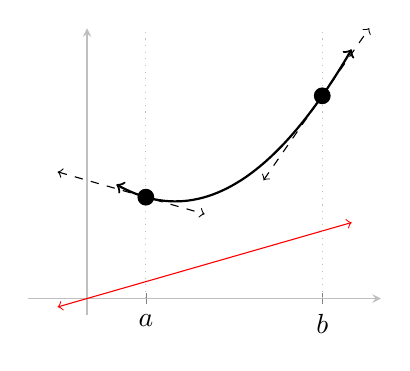
\begin{tikzpicture}
			\begin{axis}[
			xmin=-0.5,xmax=2.5,
			ymin=-0.25,ymax=4,
			xtick={0.5,2},
			ytick={0},
			xticklabels={$a$, $b$},
			yticklabels={},
			axis lines=middle,
			axis line style=lightgray,
			width=0.5\textwidth
			]
			\addplot[black,thick,<->] expression[domain=0.25:2.25,samples=50]{(x-1)^2+1 + x/2}; 
			
			
			\addplot[red,<->] expression[domain=-0.25:2.25,samples=2]{x/2}; 
			
			
			\addplot[dashed,<->] expression[domain=-0.25:1,samples=2]{-0.5*(x-0.5) + 1.5};
			\addplot[dashed,<->] expression[domain=1.5:2.4,samples=2]{2.5*(x-2) + 3}; 
			
			\addplot +[mark=none,lightgray,dotted] coordinates {(0.5, 0) (0.5, 4)};
			\addplot +[mark=none,lightgray,dotted] coordinates {(2, 0) (2, 4)};
			
			
			\node[color=black,draw=black,circle,fill,inner sep=2pt] at (axis cs:0.5,1.25+0.25) {}; 
			\node[color=black,draw=black,circle,fill,inner sep=2pt] at (axis cs:2,2+1) {}; 
			\end{axis}
			\end{tikzpicture}\hspace{1cm}
			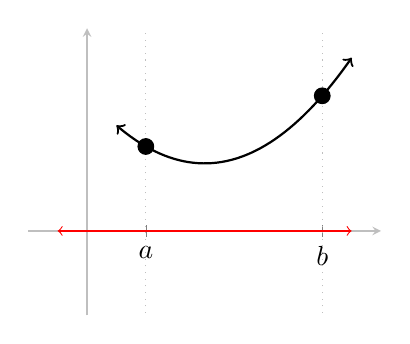
\begin{tikzpicture}
			\begin{axis}[
			xmin=-0.5,xmax=2.5,
			ymin=-1.25,ymax=3,
			ytick={0},
			xtick={0.5,2},
			xticklabels={$a$, $b$},
			yticklabels={},
			axis lines=middle,
			axis line style=lightgray,
			width=0.5\textwidth
			]
			\addplot[black,thick,<->] expression[domain=0.25:2.25,samples=50]{(x-1)^2+1}; 
			
			\addplot[red,<->] expression[domain=-0.25:2.25,samples=2]{0};
			
			\addplot +[mark=none,lightgray,dotted] coordinates {(0.5, -2) (0.5, 3)};
			\addplot +[mark=none,lightgray,dotted] coordinates {(2, -2) (2, 3)};
			
			\node[color=black,draw=black,circle,fill,inner sep=2pt] at (axis cs:0.5,1.25) {}; 
			\node[color=black,draw=black,circle,fill,inner sep=2pt] at (axis cs:2,2) {}; 
			\end{axis}
			\end{tikzpicture}
		\end{center}
		\caption{On the left is depicted the graph of a function $f$, the two tangent lines at $a$ and $b$, and the graph of the line $\ell(x) = mx$ for some $m$ in between $f'(a)$ and $f'(b)$. Subtracting $\ell$ from this picture yields the picture on the right.}  \label{subtracting-a-line}
	\end{figure}
	
	If $c = a$ were the minimum of $g$ on $[a,b]$, then we would have 
	\[ \frac{g(a+h)-g(a)}{h} > 0 \]
	for all sufficiently small positive values of $h$. This would mean that \[ f'(a) - m = g'(a) = \lim_{h \to 0^+} \frac{g(a+h)-g(a)}{h} \geq 0, \] which is a contradiction since $f'(a) < m$. Similarly, if $c = b$ were the minimum of $g$ on $[a,b]$, then we would have
	\[ \frac{g(b+h)-g(b)}{h} < 0 \]
	for all sufficiently small negative values of $h$. This would imply that 
	\[ f'(b) - m = g'(b) = \lim_{h \to 0^-} \frac{g(b+h)-g(b)}{h} \leq 0, \]
	which again is a contradiction since $m < f'(b)$. Thus we conclude that $c \in (a,b)$.  
	
	If instead we had $f'(a) > m > f'(b)$, we would define $c$ to be the point in $[a,b]$ where $g$ attains its \emph{maximum}. A similar argument then shows that $c$ must be an interior point. 
\end{proof}

\subsection{Inverse function theorem}

\begin{theorem} \label{inverse-function-theorem-single}
	Suppose that $I$ is an open interval, that $f : I \to \R$ is differentiable, and that $f'(x) \neq 0$ for all $x \in I$. Then $f$ is strictly monotone, the inverse function $f^{-1} : f(I) \to \R$ is differentiable, and 
	\[ (f^{-1})'(y) = \frac{1}{f'(f^{-1}(y))} \]
	for all $y \in f(I)$. 
\end{theorem}

\begin{proof}
	\Cref{nonzero-derivative-implies-strictly-monotone} tells us that $f$ is strictly monotone, and then \cref{strictly-monotone-implies-open} tells us that $f(I)$ is an open interval and that $f$ is open, ie, that $f^{-1}$ is continuous. To see that $f^{-1}$ is actually differentiable, fix $y \in f(I)$ and let $x = f^{-1}(y)$. For each $k$, define \[ h(k) = f^{-1}(y + k) - f^{-1}(y). \]
	Rearranging, this is equivalent the following. 
	\[ \begin{aligned} f^{-1}(y + k) &= f^{-1}(y) + h(k) \\
	f^{-1}(y + k) &= x + h(k) \\
	y + k &= f(x + h(k)) \\
	k &= f(x + h(k)) - y \\
	k &= f(x+h(k)) - f(x) \end{aligned} \]
	Thus, for any nonzero $k$, we have
	\[ \frac{f^{-1}(y + k) - f^{-1}(y)}{k} = \frac{h(k)}{k} = \frac{h(k)}{f(x + h(k)) - f(x)} = \frac{1}{ \left( \dfrac{f(x + h(k)) - f(x)}{h(k)} \right) } \]
	where for last step, we have used the fact that $h(k) \neq 0$ for all nonzero $k$ since $f^{-1}$ is injective. Since $f^{-1}$ is continuous at $y$, we have $h(k) \to 0$ as $k \to 0$. Thus the denominator on the far right above tends to $f'(x) = f'(f^{-1}(y))$ as $k \to 0$. Since the limit of the denominator is nonzero by assumption, the result follows from the quotient rule for limits. 
\end{proof}

\begin{exercise}[Power rule for fractional exponents] \label{power-rule-fractional} \index{power rule}
	Extend the result of \cref{power-rule-integer} to arbitrary rational exponents (ie, to exponents that can be written in the form $m/n$ where $m$ and $n$ are both integers). 
\end{exercise}

\begin{exercise} \label{derivative-log-proof}
	If $f(x) = \ln(x)$, prove that $f'(x) = 1/x$. You can use the facts that $\ln : (0, \infty) \to \R$ is the inverse of the exponential function, and that the exponential function is its own derivative. 
\end{exercise}

\subsection{Uniform limits \starred} \label{uniform-limit}

Derivatives interact somewhat strangely with limits. First off, here is an example to show that uniform limits of differentiable functions need not be differentiable. 

\begin{exercise}
	For any positive integer $n$, let $f_n : \R \to \R$ be the function
	\[ f_n(x) = \sqrt{x^2 + \frac{1}{n}}. \]
	\begin{enumerate}[(a)]
		\item Show that $f_n$ is differentiable. 
		\item Show that the $f_n$ converge uniformly to the absolute value function $f(x) = |x|$. 
		\item Show that the derivatives $f_n'$ converge pointwise but \emph{not} uniformly. 
	\end{enumerate}
\end{exercise}

In fact, even if a uniform limit of differentiable functions is differentiable, we cannot guarantee that the derivative of the limit is the limit of the derivatives; in fact, the derivatives need not converge at all.  

\begin{exercise}
	For any positive integer $n$, let $f_n : \R \to \R$ be the function 
	\[ f_n(x) = \frac{\sin(nx)}{n}. \]
	\begin{enumerate}[(a)]
		\item Show that $f_n$ is differentiable. 
		\item Show that the $f_n$ converge uniformly to 0. 
		\item Show that the derivatives $f_n'$ do \emph{not} converge pointwise. 
	\end{enumerate}
\end{exercise}

As suggested by part (c) of the previous two exercises, what we really need in order to have well-behaved interaction between limits and derivatives is uniform convergence \emph{of the derivatives}, rather than of the functions themselves. 

\begin{theorem} \label{differentiation-uniform-limit}
	Suppose $U$ is an open subset of $\R$ and $f_n : U \to \R$ is a differentiable function for each $n = 0, 1, \dotsc$ such that $\lim f_n = f$ pointwise. If the derivatives $f_n'$ converge uniformly on compact subsets of $U$, then $f$ is differentiable and $\lim f_n' = f'$. 
\end{theorem}

\begin{proof}
	Set $g = \lim f_n'$. Fix $a \in U$ and consider the following ``slope of secant'' functions (as in the first proof of the chain rule in \cref{chain-rule-single-section}). 
	\[ \begin{aligned} \sigma_n(h) &= \begin{cases} \dfrac{f_n(a+h) - f_n(a)}{h} & \text{if } h  \neq 0 \\ f_n'(a) & \text{if } h = 0 \end{cases} \\ 
	\sigma(h) &= \begin{cases} \dfrac{f(a+h) - f(a)}{h} & \text{if } h  \neq 0 \\ g(a) & \text{if } h = 0 \end{cases} \end{aligned} \]
	Continuity of $\sigma_n$ and $\sigma$ away from $h = 0$ is clear. At $h = 0$, we know that $\sigma_n$ is continuous because $f_n$ is differentiable at $a$. Note moreover that $\sigma_n$ converges pointwise to $\sigma$. 
	
	If we can show that $\sigma$ is continuous at $0$, then $f$ is differentiable at $a$ and $f'(a) = g(a) = \lim f_n'(a)$, which is what we ultimately want to prove. To show that $\sigma$ is continuous at 0, our strategy is to prove that $\sigma_n$ converges \emph{uniformly} to $\sigma$ on a compact interval $I$ containing 0 (not just pointwise, which we've already observed above). Then we can invoke the theorem guaranteeing that uniform limits of continuous functions are continuous (cf. \cite[theorem 9.13]{protter-morrey}) in order to conclude that $\sigma$ is continuous.
	
	Observe that for any pair of integers $m, n$ and any $h \in I \setminus \{0\}$, we have
	\[ \sigma_m(h) - \sigma_n(h) = \frac{(f_m(a+h) - f_n(a+h)) - (f_m(a) - f_n(a))}{h} = f_m'(\xi) - f_n'(\xi), \]
	where for the last step we have applied the mean value theorem to the function $f_m - f_n$ on the closed interval between $a$ and $a + h$ to find $\xi$ strictly between $a$ and $a + h$. Moreover, we have $\sigma_m(0) - \sigma_n(0) = f_m'(a) - f_n'(a)$. In other words, if we set $J = \{a + x : x \in I\}$, then for every $h \in I$, there exists $\xi \in J$ such that $\sigma_m(h) - \sigma_n(h) = f_m'(\xi) - f_n'(\xi)$, which implies that
	\[ \|\sigma_m - \sigma_n\|_{\spn, I} \leq \|f_m' - f_n'\|_{\spn, J}. \]
	Since the derivatives converge uniformly on the compact interval $J$, they are uniformly Cauchy. It follows from the above inequality that the $\sigma_n$ are also uniformly Cauchy, and therefore uniformly convergent. Since $\sigma$ is the pointwise limit of the $\sigma_n$, it must also be the uniform limit; in other words, we have now proved that $\sigma_n$ converges uniformly to $\sigma$, as we wanted. 
\end{proof}

\begin{unimportantremark}
	The hypotheses of this theorem can be made weaker by only assuming that the functions $f_n$ converge \emph{just at a single point} rather than pointwise on all of $U$, but one still needs to assume uniform convergence of the derivatives on compact subsets \cite[theorem 7.17]{rudin}. The idea of the proof of this generalization is similar to the proof above, but the flow of the argument gets obscured by more technical details. 
\end{unimportantremark}

% TODO: Convergence of the functions themselves is uniform.

This theorem lets us prove that we can differentiate power series term-by-term.

\begin{theorem} \label{differentiating-power-series}
	Suppose the power series $\sum_{n = 0}^\infty a_n x^n$
	has a nonzero radius of convergence $R$. Then the function $f : (-R, R) \to \R$ given by
	\[ f(x) = \sum_{n = 0}^\infty a_n x^n \]
	is differentiable and
	\[ f'(x) = \sum_{n = 0}^\infty na_n x^{n-1}. \]
	Moreover, the radius of convergence of the power series $\sum_{n = 0}^\infty na_n x^{n-1}$
	is also $R$. 
\end{theorem}

\begin{proof}
	Let 
	\[ f_n(x) = a_0 + a_1 x + \dotsb + a_n x^n \]
	be the sequence of the partial sums of the power series. Then clearly $\lim f_n = f$ pointwise. The conclusion of \cref{differentiating-power-series} would therefore follow by applying \cref{differentiation-uniform-limit} to the sequence $f_n$, provided we first show that $f_n'$ converges uniformly on compact subsets of $(-R, R)$. To prove this, it is sufficient to show that the radius of convergence of the power series 
	\[ \sum_{n = 0} na_n x^{n-1} \]
	is also $R$. Let $R'$ denote the radius of convergence of this power series; we want to show that $R' = R$. We also know that
	\[ \frac{1}{R} = \limsup_{n \to \infty} |a_n|^{1/n}.  \] 
	Observe that
	\[ \frac{1}{R'} = \limsup_{n \to \infty} |na_n|^{1/(n-1)} = \limsup_{n \to \infty} (|na_n|^{1/n})^{n/(n-1)}. \]
	Since $\lim n^{1/n} = 1$ and $\lim n/(n-1) = 1$, we conclude that $R = R'$. 
\end{proof}

\begin{exercise}
	Verify that, if the exponential, sine, and cosine functions are defined by their power series as in \cref{exp-sin-cos-power-series}, then their derivatives are calculated by the formulas we stated in \cref{non-rational}. 
\end{exercise}

\begin{comment}
%TODO: Bizarre differentiable functions \starred

This section is just for fun: we'll discuss many bizarre examples of differentiable functions. We'll start off with the following variant of a function we saw in \cref{power-times-sine}. 

\begin{exercise} \label{power-times-sine-truncated}
	Consider the function $f : \R \to \R$ defined as follows.
	\[ f(x) = \begin{cases} x^2 \sin(1/x) & \text{if } x >  0 \\ 0 & \text{if } x \leq 0 \end{cases} \]
	\begin{enumerate}[(a)]
		\item Show that $f$ is differentiable, and that
		\[ f'(x) = \begin{cases} 2x\sin(1/x) - \cos(1/x) & \text{if } x > 0 \\ 0 & \text{if } x \leq 0 \end{cases}. \]
		\item Show that $f'$ is continuous everywhere except at 0. 
		\item Show that $|f'(x)| \leq 3$ for all $x \leq 1$. 
	\end{enumerate}
\end{exercise}

\begin{example}
	Consider the function $h : \R \to \R$ defined as follows.
	\[ h(x) = \begin{cases} (1 - x^2)^2 \sin\left(\dfrac{1}{1 - x^2} \right) & \text{if } x \in (-1,1) \\ 0 & \text{otherwise} \end{cases} \]
	If $f : \R \to \R$ is the function from \cref{power-times-sine-truncated} and $g(x) = 1 - x^2$, observe that $h = f \circ g$. It follows from the chain rule \ref{chain-rule-single} that $h$ is differentiable and
	\[ h'(x) = f'(g(x)) g'(x). \]
	Since $f'$ is continuous everywhere except 0, we see that $h'$ is also continuous everywhere except when $g(x) = 0$, ie, when $x = \pm 1$. 
	
	We know that $h'(x) = 0$ on $(-\infty, -1]$ and $[1, \infty)$. On $(-1,1)$, observe that $0 < g(x) \leq 1$ and $|g'(x)| < 2$. Using the bound from the final part of \cref{power-times-sine-truncated}, 
	\[ |h'(x)| = |f'(g(x))||g'(x)| \leq 6. \]
	Thus $\|h'\|_\spn$ is finite. 
\end{example}

\begin{exercise} \label{derivative-discontinuous-two-points}
	For any $a < b$ in $\R$, construct a differentiable function $h : \R \to \R$ supported\footnotemark\ on $[a,b]$ such that $\|h'\|_{\spn} = 1$ and $h'$ is continuous everywhere except at $a$ and $b$. 
\end{exercise}

\footnotetext{Recall that the \emph{support}\index{support} of a function is the closure of the subset of its domain where it takes nonzero values.}

\begin{example}[Volterra]
	Let $F$ be a closed subset of $\R$ with empty interior. Then the complement of $F$ is an open subset of $\R$, so
	\[ \R \setminus F = \bigcup_{n = 0}^\infty (a_n, b_n) \]
	where the open intervals $(a_n, b_n)$ are all disjoint (cf. \cite[theorem 6.17]{protter-morrey}). Use \cref{derivative-discontinuous-two-points} to construct a differentiable function $h_n : \R \to \R$ supported on $[a_n, b_n]$ which is discontinuous at $a_n$ and $b_n$. Then consider the function
	\[ h(x) = \sum_{n = 0}^\infty \frac{h_n(x)}{2^n}. \] 
	This looks like an infinite series, but it's not. Every $x \in \R$ is either in $F$, in which case $h(x) = 0$, or there exists a unique integer $n$ such that $x \in (a_n, b_n)$, in which case $h(x) = h_n(x)/2^n$. Then $h$ is differentiable and $h'$ is discontinuous at all of the $a_0, b_0, a_1, b_1, \dotsc$. 
\end{example}
\end{comment}

\section{\texorpdfstring{$C^k$}{Ck} hierarchy} 

\subsection{Continuous differentiability}

We saw in \cref{darboux-section} that the derivative of a differentiable function is always ``close'' to being continuous, though in a slightly bizarre way. Insisting that the derivative actually be continuous is often useful for ruling out pathological behavior. 

\begin{definition}
	Suppose $U$ is an open subset of $\R$ and $f : U \to \R$ is differentiable. If the derivative $f' : U \to \R$ is also continuous, then $f$ is said to be \emph{continuously differentiable}.\index{continuously differentiable} 
\end{definition}

Here is an important ``reasonableness'' property of continuously differentiable functions. 

\begin{exercise} \label{critical-locus-closed-single}
	Show that, if $f : U \to \R$ is continuously differentiable, then the set
	\[ C = \{ x \in U : f'(x) = 0 \} \]
	is a closed subset of $U$. 
\end{exercise}

\Cref{critical-locus-closed-single} actually tells us that lots of strange pathological behavior is ruled out by insisting that the derivative is continuous. For example, we saw in \cref{positive-not-monotone} that $f(x) = x + 2x^2\sin(1/x)$ defined a differentiable function $f : \R \to \R$ such that $f'(0) \neq 0$, but which is not monotone on any interval containing that point. This is rather bizarre behavior, and it cannot happen with continuously differentiable functions. 

\begin{exercise} \label{nonzero-derivative-at-point-implies-monotone-in-neighborhood}
	Suppose $f : U \to \R$ is continuously differentiable, and $a \in U$ is a point such that $f'(a) \neq 0$. Use \cref{critical-locus-closed-single} to conclude that there exists an open interval containing $a$ on which $f$ is strictly monotone. 
\end{exercise}

To appreciate the following fact, it's worth noting the following: there exist \emph{non-constant} differentiable functions $f : U \to \R$ such that $f'(x) = 0$ for all $x \in U \cap \Q$! These extremely bizarre functions were first found by Pompeiu \cite{pompeiu}. This pathological behavior is also ruled out by insisting that the derivative be continuous. 

\begin{exercise} \label{critical-dense-implies-constant}
	Suppose $f : U \to \R$ is continuously differentiable. Use \cref{critical-locus-closed-single} to show that, if $f'(x) = 0$ for all $x \in U \cap \Q$, then $f$ is constant. 
\end{exercise}

Unfortunately, insisting that the derivative of a function be continuous does not rule out all possible bizarre behavior. For example, in \cref{extremum-no-sign-change}, we saw that $f(x) = x^4 \left( 2 + \sin(1/x) \right)$ defined a differentiable function $f$ with an absolute minimum at 0, but the derivative doesn't just simply ``change sign'' at 0. In fact, it turns out that function is also continuously differentiable (cf. \cref{extremum-no-sign-change-continued}), so merely insisting on continuous differentiability does not quite manage to rule out that kind of pathological behavior. However, as it turns out, the derivative of $f'$ (called the ``second derivative'' of $f$, and denoted $f''$), turns out \emph{not} to be continuous. 

\begin{exercise} \label{extremum-no-sign-change-continued}
	Let $f : \R \to \R$ be the function from \cref{extremum-no-sign-change}. Show that $f'$ is differentiable (so, in particular, $f$ is continuously differentiable), but that $f''$ is not continuous. 
\end{exercise}

This leads us to thinking about iterated derivatives. 

\subsection{\texorpdfstring{$C^k$}{Ck} functions}

\begin{definition} \label{ck-single} \index{ck@$C^k$}
	Let $U$ be an open subset of $\R$ and $f : U \to \R$ a function. We then define the following. 
	\begin{itemize}
		\item $f$ is said to be $C^0$ if it is continuous. 
		\item $f$ is said to be $C^1$ if it is continuously differentiable. 
		\item $f$ is said to be $C^2$ if it is differentiable and $f'$ is $C^1$. In this case, the derivative $(f')'$ of $f'$ is called the \emph{second derivative} of $f$, and is denoted either $f''$ or $f^{(2)}$. 
		\item $f$ is said to be $C^3$ if it is differentiable and $f'$ is $C^2$.  In this case, the second derivative $(f')''$ of $f'$ is called the \emph{third derivative} of $f$ and is denoted $f^{(3)}$. 
		\item $f$ is said to be $C^4$ if it is differentiable and $f'$ is $C^3$.  In this case, the third derivative $(f')^{(3)}$ of $f'$ is called the \emph{fourth derivative} of $f$ and is denoted $f^{(4)}$. 
	\end{itemize}
	Inductively, for any positive integer $k$, $f$ is said to be $C^k$ if it is differentiable and $f'$ is $C^{k-1}$.  In this case, the $(k-1)$st derivative $(f')^{(k-1)}$ of $f'$ is called the \emph{$k$th derivative} of $f$ and is denoted $f^{(k)}$.  
\end{definition}

First up, let's prove that all reasonable ways of combining functions in a particular differentiability class stays within that differentiability class. 

\begin{exercise} \label{ck-stable-sum-scalar-single}
	Prove that the set of all $C^k$ functions $U \to \R$ is a vector space. 
	\begin{hint}
		Induct on $k$. 
	\end{hint}
\end{exercise}

\begin{exercise} \label{ck-stable-product-single}
	\begin{enumerate}[(a)]
		\item Prove that the product of any two $C^k$ functions is also $C^k$. 
		\item If $f, g : U \to \R$ are $C^k$ functions, show that
		\[ (fg)^{(k)} = \sum_{i = 0}^k \binom{k}{i} f^{(i)} g^{(k-i)}. \]
	\end{enumerate}
\end{exercise}

\begin{exercise} \label{ck-stable-composite-single}
	Show that the composite of two $C^k$ functions is also $C^k$. \begin{hint} Induct on $k$. The base case $k = 0$ is clear. For the inductive step, use the chain rule \ref{chain-rule-single} and \cref{ck-stable-product-single}(a). \end{hint}
\end{exercise}

\begin{exercise} \label{ck-stable-reciprocal-single}
	Suppose $f : U \to \R$ is $C^k$ and $f(x) \neq 0$ for all $x \in U$. Show that $1/f$ is also $C^k$.
	\begin{hint}
		You might first show that the function $g(x) = 1/x$ is $C^k$ for all $k$. Then $1/f = g \circ f$, so you can apply \cref{ck-stable-composite-single}. 
	\end{hint}
\end{exercise}

\begin{proposition} \label{ck-stable-inversion-single}
	Suppose $I$ is an open interval, $f : I \to \R$ is injective, $C^k$ for some $k \geq 1$, and that $f'(x) \neq 0$ for all $x \in I$. Then $f^{-1} : f(I) \to U$ is also $C^k$. \index{inverse function}
\end{proposition}

\begin{proof}
	Since $f'$ is nonzero on $I$, we know from \cref{inverse-function-theorem-single} that $f^{-1}$ is differentiable and that
	\[ (f^{-1})'(a) = \frac{1}{f'(f^{-1}(a))}. \]
	In other words, $(f^{-1})'$ is the composite of three functions: $f^{-1}$, $f'$, and the function $x \mapsto 1/x$. 
	
	We will inductively prove that $f^{-1}$ is $C^r$ for all $0 \leq r \leq k$. Certainly $f^{-1}$ is $C^0$ (ie, continuous), since it is even differentiable, as we saw above. Inductively, suppose $f^{-1}$ is $C^r$ for some $0 \leq r < k$. We know that $f$ is $C^k$ and therefore $C^r$, and also that $x \mapsto 1/x$ is $C^r$ (cf. \cref{ck-stable-reciprocal-single}), so $(f^{-1})'$ is the composite of three $C^r$ functions. Thus \cref{ck-stable-composite-single} tells us that $(f^{-1})'$ is $C^r$, which shows that $f^{-1}$ is $C^{r+1}$. This completes the induction.  
\end{proof}

Observe that \cref{differentiable-implies-continuous-single} tells us that we have an infinite chain of implications
\[ \dotsb \implies C^3 \implies C^2 \implies C^1 \implies C^0. \]
The following shows that all of these implications are strict; in other words, for every $k$, there exists a $C^k$ function which is not $C^{k+1}$.

\begin{exercise}
	For any non-negative integer $k$, let 
	\[ f_k(x) = x^k|x|. \]
	See \cref{power-times-absolute-value-graphs}. Prove that $f_k$ is $C^k$, but the $(k+1)$st derivative $f^{(k+1)}$ does not exist. \begin{hint} First prove that $f_{k+1}' = (k+2)f_k$. \end{hint}
	
	\begin{figure}[ht]
		\begin{center}
			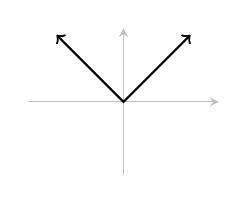
\begin{tikzpicture}
			\begin{axis}[
			xmin=-1.1,xmax=1.1,
			ymin=-1.1,ymax=1.1,
			xtick={0},
			ytick={0},
			axis lines=middle,
			axis line style=lightgray,
			width=0.33\textwidth,
			axis equal
			]
			\addplot[black,style=thick,<->] expression[domain=-1:1,samples=3]{abs(x)}; 
			
			\end{axis}
			\end{tikzpicture}
			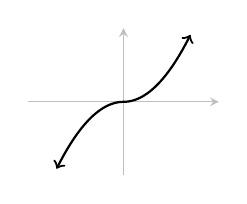
\begin{tikzpicture}
			\begin{axis}[
			xmin=-1.1,xmax=1.1,
			ymin=-1.1,ymax=1.1,
			xtick={0},
			ytick={0},
			axis lines=middle,
			axis line style=lightgray,
			width=0.33\textwidth,
			axis equal
			]
			\addplot[black,style=thick,<->] expression[domain=-1:1,samples=50]{x*abs(x)}; 
			
			\end{axis}
			\end{tikzpicture}
			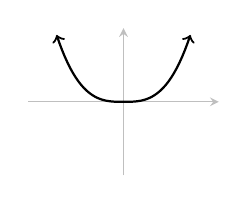
\begin{tikzpicture}
			\begin{axis}[
			xmin=-1.1,xmax=1.1,
			ymin=-1.1,ymax=1.1,
			xtick={0},
			ytick={0},
			axis lines=middle,
			axis line style=lightgray,
			width=0.33\textwidth,
			axis equal
			]
			\addplot[black,style=thick,<->] expression[domain=-1:1,samples=50]{x^2*abs(x)}; 
			
			\end{axis}
			\end{tikzpicture}
			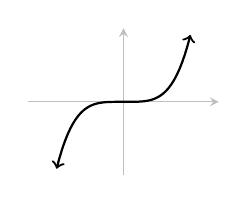
\begin{tikzpicture}
			\begin{axis}[
			xmin=-1.1,xmax=1.1,
			ymin=-1.1,ymax=1.1,
			xtick={0},
			ytick={0},
			axis lines=middle,
			axis line style=lightgray,
			width=0.33\textwidth,
			axis equal
			]
			\addplot[black,style=thick,<->] expression[domain=-1:1,samples=50]{x^3*abs(x)}; 
			
			\end{axis}
			\end{tikzpicture}
		\end{center}
		\caption{Graphs of the functions $f_k(x) = x^k|x|$ for $k = 0, 1, 2, 3$.} \label{power-times-absolute-value-graphs}
	\end{figure}
\end{exercise}

\begin{exercise}
	For any positive integer $k$, let $f_k : \R \to \R$ be the function given by
	\[ f_k(x) = \begin{cases} x^{k+1} \sin(1/x) &  \text{if } x \neq 0 \\ 0 & \text{if } x = 0. \end{cases} \]
	Show that the $k$th derivative $f^{(k)}$ exists, but it is not continuous. 
\end{exercise}

Here is a property of $C^2$ functions you likely recognize from calculus. 

\begin{exercise} \label{second-derivative-concavity}
	Suppose $I$ is an open interval and $f : I \to \R$ is $C^2$. 
	\begin{enumerate}[(a)]
		\item Show that $f$ is concave up if and only if $f'' \geq 0$.
		\item Show that $f$ is concave down if and only if $f'' \leq 0$.  
	\end{enumerate}
\end{exercise}

\begin{exercise} \label{second-derivative-strict-concavity}
	Suppose $I$ is an open interval and $f : I \to \R$ is $C^2$. 
	\begin{enumerate}[(a)]
		\item Show that, if $f'' > 0$, then $f$ is strictly concave up.
		\item Show that, if $f'' < 0$, then $f$ is strictly concave down. 
		\item Unlike \cref{second-derivative-concavity}, the above two statements cannot be upgraded to ``if and only if'' statements. Give an example of a strictly concave up function $f : \R \to  \R$ for which there exists some $a \in \R$ such that $f''(a) = 0$. 
	\end{enumerate}
\end{exercise}

\subsection{Taylor's theorem \starred}

Taylor's theorem gives us a way of approximating a $C^k$ function by a polynomial of at most degree $k$. When $k = 1$, the theorem says nothing more than \cref{differential-unique-single}.

\begin{theorem}[Taylor] \label{taylor-single}
	Suppose $I$ is an open interval, $f : I \to \R$ is $C^k$ for some non-negative integer $k$, and $a \in I$. Then there exists a unique polynomial $p_k$ at most $k$, called the \emph{degree $k$ Taylor polynomial of $f$ at $a$}, such that $|f(a+h) - p_k(h)| = o(|h|^k)$ as $h \to 0$. Moreover, we have
	\begin{equation} \label{taylor-polynomial-single} p_k(h) = f(a) + f'(a)h + \frac{f''(a)}{2!}h^2 + \frac{f^{(3)}(a)}{3!} h^3 + \dotsb + \frac{f^{(k)}(a)}{k!} h^k. \end{equation}
\end{theorem}

\begin{proof}
	Let $p_k(h)$ be defined as \cref{taylor-polynomial-single} and set $r(h) = f(a+h) - p_k(h)$. Observe that $r$ is $C^k$ by \cref{ck-stable-sum-scalar-single}. By direct calculation, we have $r^{(i)}(0) = 0$ for all $i = 0, 1, \dotsc, k$. If $k = 0$, then the fact that $|r(h)| = o(1)$ follows from the continuity (ie, $C^0$-ness) of $r$ and the fact that $r(0) = 0$; so we can assume for the rest of the proof that $k \geq 1$. 
	
	Suppose $h > 0$. By iterating the mean value theorem, we have
	\[ \begin{aligned} r(h) &= r(h) - r(0) \\
	&= r'(h_1)h = (r'(h_1) - r'(0))h \\
	&= r''(h_2)h_1 h = (r''(h_2) - r''(0))h_1 h \\
	&\enspace\vdots\\
	&= r^{(k-1)}(h_{k-1}) h_{k-2} h_{k-3} \dotsb h_2 h_1 h \end{aligned} \]
	where $0 < h_{k-1} < \dotsb < h_2 < h_1 < h$. This means that
	\[ \begin{aligned} \frac{|r(h)|}{|h|^k} &= \left| \frac{r^{(k-1)}(h_{k-1}) h_{k-2} \dotsb h_2 h_1 h}{h^k} \right| \\
	&\leq \left| \frac{r^{(k-1)}(h_{k-1}) h^{k-1}}{h^k} \right| \\
	&= \left| \frac{r^{(k-1)}(h_{k-1})}{h} \right| \\
	&\leq \left| \frac{r^{(k-1)}(h_{k-1})}{h_{k-1}} \right| \\
	&= \left| \frac{r^{(k-1)}(h_{k-1}) - r^{(k-1)}(0)}{h_{k-1}} \right|. \end{aligned}  \]
	Now as $h \to 0^+$, we also have that $h_{k-1} \to 0$, so this final expression tends to $r^{(k)}(0) = 0$. By the squeeze theorem, we conclude that 
	\[ \lim_{h \to 0^+} \frac{|r(h)|}{|h|^k} = 0. \]
	One argues similarly with $h < 0$ to prove that
	\[ \lim_{h \to 0^-} \frac{|r(h)|}{|h|^k} = 0. \]
	In this case, we have $h < h_1 < h_2 < \dotsb < h_{k-1} < 0$. This proves that $|r(h)| = o(|h|^k)$.
	
	To prove that $p_k$ is unique, suppose $q$ is any polynomial of degree at most $k$ such that $|f(a+h) -q(h)| = o(|h|^k)$. Then 
	\[ |p_k(h) - q(h)| \leq |f(a+h) - p_k(h)| + |f(a+h) - q(h)| \] 
	so \cref{little-o-vector-space,less-than-small-is-small} imply that $|p_k(h) -  q(h)| = o(|h|^k)$. But $p_k - q$ is a polynomial of degree at most $k$, and a nonzero polynomial of degree at most $k$ cannot be $o(|h|^k)$ as $h \to 0$. So we must have $p_k = q$.
\end{proof}

\begin{unimportantremark}
	It's worth remarking that Taylor's theorem does not use the fact that $f^{(k)}$ is continuous; it merely requires that $f^{(k)}$ exists, ie, that $f$ is \emph{$k$ times differentiable}. This is evident in the proof above. 
\end{unimportantremark}

The difference 
\[ r(h) = f(a+h) - p_k(h) \]
is often called a ``remainder,''\index{remainder} since it's what's left over after we approximate $f$ by its Taylor polynomial. When $k = 1$, this is precisely the remainder function we discussed in \cref{remainder-linear}.

\begin{exercise}[L'H\^opital's rule, less weak version] \label{lhopital-less-weak}
	Suppose $f, g : U \to \R$ are $C^k$ functions for some $k \geq 1$ and 
	\[ \begin{aligned} f(a) = f'(a) = \dotsb = f^{(k-1)}(a) = 0 \\
	g(a) = g'(a) = \dotsb = g^{(k-1)}(a) = 0 \end{aligned} \]
	and $g^{(k)}(a) \neq 0$. Prove that 
	\[ \lim_{x \to a} \frac{f(x)}{g(x)} = \frac{f^{(k)}(a)}{g^{(k)}(a)}. \]
	\begin{hint}
		Mimic the proof of \cref{lhopital-weak}, but now use $r(h) = f(a+h) - p_k(h)$ instead of $r(h) = f(a+h) - p_1(h)$. 
	\end{hint}
\end{exercise}

\begin{exercise}
	Suppose $f : U \to \R$ is $C^2$ and $a \in U$ is a point such that $f'(a) = 0$. 
	\begin{enumerate}[(a)]
		\item Show that, if $f''(a) > 0$, then $a$ is a strict local minimum of $f$, and that if $f''(a) < 0$, then $a$ is a strict local maximum of $f$. 
		\begin{hint}
			You can do this using \cref{concavity-extremums,second-derivative-strict-concavity}. Alternatively, you can do it using Taylor's theorem \ref{taylor-single}. Try both methods. It's the Taylor's theorem method that will be more helpful for part (c) below. You may also notice that the first method really requires that $f$ be $C^2$, while the Taylor's theorem method only requires that $f$ be twice differentiable. 
		\end{hint}
	
		\item Give examples to show that, if $f''(a) = 0$, then the test from part (a) is entirely inconclusive: $a$ could be a strict local extremum (of either type), a non-strict local extremum (of either type), or not a local extremum at all. 
		
		\item Suppose $f$ is $C^k$ for some $k \geq 2$, that 
		\[ f'(a) = f^{(2)} = \dotsb = f^{(k-1)}(a) = 0 \]
		and that $f^{(k)}(a) \neq 0$. Formulate and prove a rule that uses the sign of $f^{(k)}(a)$ and/or the parity of $k$ to determine whether or not $a$ is a local extremum, and if it is a local extremum, what kind of local extremum it is. 
	\end{enumerate}
\end{exercise}

We now return to our discussion of the pathology exhibited by the function $f(x) = x^4 \left( 2 + \sin(1/x) \right)$ from \cref{extremum-no-sign-change,extremum-no-sign-change-continued}, which has the strange property that $f'(0) = 0$ but $f$ is not monotone on any interval to the left or to the right of 0. Such pathologies cannot occur if the function eventually has a nonzero derivative. 

% We prepare for this discussion with the following lemma. 
\begin{comment}
\begin{lemma} \label{eventual-nonvanishing-derivative}
	Suppose $I$ is an open interval, $f : I \to \R$ is $C^k$ for some positive integer $k$, that 
	\[ f(a) = f'(a) = f^{(2)}(a) = \dotsb = f^{(k-1)}(a) = 0, \] and that $f^{(k)}(a) > 0$. Then there exists an $\epsilon > 0$ such that $f$ is positive on $(a, a+\epsilon)$, and on $(a-\epsilon, a)$, $f$ is positive if $k$ is even and negative if $k$ is odd. Moreover, if $f^{(k)}(a) < 0$, then all instances of ``positive'' in the conclusion get replaced by ``negative'' and vice versa. 
\end{lemma}

\begin{proof}
	Let us suppose that $f^{(k)}(a) > 0$. By Taylor's theorem \ref{taylor-single}, we see that
	\[ f(a+h) = \frac{f^{(k)}(a)}{k!} h^k + r(h) \]
	where $|r(h)| = o(|h|^k)$ as $h \to 0$. Dividing through by $h^k$, we see that 
	\[ \frac{f(a+h)}{h^k} = \frac{f^{(k)}(a)}{k!} + \frac{r(h)}{h^k}. \]
	Since $f^{(k)}(a) > 0$, we also have $f^{(k)}(a)/k! > 0$. Since $\lim_{h \to 0} |r(h)/h^k| = 0$, there exists $\epsilon > 0$ such that $|r(h)/h^k| < f^{(k)}(a)/k!$ for all $|h| < \epsilon$. Then, if $0 < |h| < \epsilon$, we have
	\[ \frac{f(a+h)}{h^k} = \frac{f^{(k)}(a)}{k!} + \frac{r(h)}{h^k} > 0. \]
	Now note that if $k$ is even, then $h^k$ is always positive, so the lemma follows. On the other hand, if $k$ is odd, then $h^k$ is positive for positive $h$ and negative for negative $h$, and again the lemma follows. The proof when $f^{(k)}(a) < 0$ is similar. 
\end{proof}
\end{comment}

\begin{exercise} \label{extremum-sign-change}
	Suppose $f$ is $C^k$ for some $k \geq 2$, that
	\[ f'(a) = f^{(2)}(a) = \dotsb = f^{(k-1)}(a) = 0 \] and $f^{(k)}(a) \neq 0$. Prove that there exists an $\epsilon > 0$ such that $f$ is strictly monotone on $(a-\epsilon, a)$ and on $(a, a+\epsilon)$. 
\end{exercise}

\begin{example} \label{extremum-no-sign-change-final}
	Let $f : \R \to \R$ be the function $f(x) = x^4(2 + \sin(1/x))$ of \cref{extremum-no-sign-change,extremum-no-sign-change-continued}. Then $f$ is twice differentiable and $f'(0) = f''(0) = 0$, but it is not thrice differentiable at 0. In other words, it doesn't eventually have a nonzero derivative at 0, so we're not able to apply \cref{extremum-sign-change}. 
\end{example}

It turns out that if $f$ is $C^{k+1}$, we can use the mean value theorem to express the remainder in terms of the $(k+1)$st derivative. 

\begin{theorem}[Taylor's theorem with remainder, Lagrange form] \label{taylor-single-remainder-lagrange}
	Suppose $I$ is an open interval, $f : I \to \R$ is $C^{k+1}$ for some non-negative integer $k$ and $a \in I$. Then for any $h$ such that $a+h \in I$, there exists $\xi$ between $a$ and $a+h$ such that 
	\[ f(a+h) - p_k(h) = \frac{f^{(k+1)}(\xi)}{(k+1)!}h^{k+1}, \]
	where $p_k$ is the degree $k$ Taylor polynomial of $f$ at $a$. 
\end{theorem}

\begin{proof}
	When $k = 0$, we have $p_0(h) = f(a)$ and the statement follows immediately from the mean value theorem \ref{mean-value-theorem}. So we can assume that $k \geq 1$. Let $r(h) = f(a+h) - p_k(h)$. Fix $h > 0$ and consider the function
	\[ g(t) = r(t) - \frac{r(h)}{h^{k+1}} t^{k+1}.  \]
	Plugging in $t = h$, we see that $g(h) = 0$. As we noted in the proof of Taylor's theorem \ref{taylor}, we have $r^{(i)}(0) = 0$ for $i = 0, 1, \dotsc, k$, from which it follows that $g^{(i)}(0) = 0$ for $i = 0, 1, \dotsc, k$. Moreover, we have \[ g^{(k+1)}(t) = f^{(k+1)}(t) - \frac{(k+1)!r(h)}{h^{k+1}},  \]
	because $p_k$ is a polynomial of degree at most $k$, which means that its $(k+1)$st derivative vanishes. 
	
	Since $g(0) = g(h) = 0$, Rolle's theorem \ref{rolles-theorem} tells us that there exists $h_1$ between $0$ and $h$ such that $g'(h_1) = 0$. Since $g'(0) = g'(h_1) = 0$, Rolle's theorem again gives us $h_2$ between $0$ and $h_2$ such that $g^{(2)}(h_2) = 0$. Inductively, we find a sequence $0 < h_{k+1} < h_k < h_{k-1} < \dotsb < h_1 < h$ such that $g^{(i)}(h_i) = 0$ for all $i = 0, \dotsc, k, k+1$. Letting $\xi = h_{k+1}$, we find that 
	\[ 0 = g^{(k+1)}(\xi) = f^{(k+1)}(\xi) - \frac{(k+1)!r(h)}{h^{k+1}}, \]
	and rearranging this equation yields precisely
	\[ f(a+h) - p_k(h) = r(h) = \frac{f^{(k+1)}(\xi)}{(k+1)!}h^{k+1}. \]
	The proof when $h < 0$ is analogous. 
\end{proof}

\subsection{Smooth functions} \label{smooth-single}

Insisting that a function be $C^k$ for larger and larger values of $k$ rules out more and more pathological behavior. This suggests the following. 

\begin{definition} \index{smooth} \index{Cinfinity@$C^\infty$|see {smooth}} \index{infinitely differentiable|see {smooth}}
	A function $f : U \to \R$ is said to be $C^\infty$, or \emph{infinitely differentiable}, or \emph{smooth}, if it is $C^k$ for all $k$. 
\end{definition}

It's a little annoying that there are three different words that all mean the same thing, but that's just how it is; all three are commonly used in the mathematical literature, so it's best to get used to all of them. We'll usually use the word ``smooth.'' 

It follows immediately from \cref{ck-stable-sum-scalar-single,ck-stable-product-single,ck-stable-reciprocal-single,ck-stable-composite-single,ck-stable-inversion-single} that sums, scalar multiples, products, reciprocals, composites, and inverses of smooth functions are also smooth. 

The class of smooth functions is very well-behaved. On the one hand, as we have already seen, smoothness rules out lots of pathological behavior. For example, functions like \cref{positive-not-monotone} are not smooth, and in fact, if the derivative of a smooth function $f$ is nonzero at a single point, then $f$ must be strictly monotone in a neighborhood of that point (cf. \cref{nonzero-derivative-at-point-implies-monotone-in-neighborhood}). We've also seen that functions like the one from \cref{extremum-no-sign-change,extremum-no-sign-change,extremum-no-sign-change-final} are not smooth, and that if $f$ is smooth and $a$ is a local extremum and eventually $f$ has a nonzero derivative at $a$, then in fact the derivative of $f$ must ``change sign'' at $a$ (cf. \cref{extremum-sign-change}). 

On the other hand, the class of smooth functions is not overly restrictive. There is a vast array of smooth functions, and we can tailor smooth functions to almost arbitrary specifications. 

\subsubsection*{Diffeomorphisms}

Our first example of this principle is the following smooth bijection $(-1,1) \to \R$ whose inverse is also smooth. A smooth bijection with a smooth inverse is also called a ``diffeomorphism.''\index{diffeomorphism} Roughly, the fact that there exists diffeomorphism $(-1,1) \to \R$ ``smoothly stretch out'' $(-1,1)$ to all of $\R$, and also ``smoothly shrink'' all of $\R$ down to $(-1,1)$. 

\begin{example} \label{interval-to-line}
	Consider the function $f : (-1,1) \to \R$ defined by \[ f(x) = \frac{x}{1-x^2}. \]
	See \cref{interval-to-line-graph}. 
	Since this is a quotient of two smooth functions and the denominator is nonzero on $(-1,1)$, this function is also smooth. We can calculate that
	\[ f'(x) = \frac{1+x^2}{(1-x^2)^2} \]
	and we can see from this formula that the derivative is always strictly positive, so $f$ is strictly increasing\index{monotone!strictly increasing} (cf. \cref{strictly-monotone-derivative}). In particular, it is injective. Moreover, we have
	\[ \lim_{x \to -1^+} f(x) = -\infty \quad \text{ and } \lim_{x \to 1^-} f(x) = +\infty \]
	so the intermediate value theorem\index{intermediate value theorem} guarantees that $f$ is bijective. Thus the inverse function $f^{-1} : \R \to (-1,1)$ exists. Finally, since $f'$ is always nonzero, it follows from \cref{ck-stable-inversion-single} that $f^{-1}$ must be smooth. It is possible to verify that
	\[ f^{-1}(x) = \frac{-1+\sqrt{4x^2+1}}{2x} \]
	by check that composing this formula with $f$ yields the identity, but, thanks to \cref{ck-stable-inversion-single}, we don't actually need this formula for $f^{-1}$ at all to know that $f^{-1}$ is smooth.
\end{example}


\begin{figure}
	\begin{center}
		\begin{tikzpicture}
		\begin{axis}[
		xmin=-1.5,xmax=1.5,
		ymin=-5,ymax=5,
		ytick={0},
		xtick={-1,1},
		xticklabels={$-1$,1},
		yticklabels={},
		axis lines=middle,
		axis line style=lightgray,
		width=0.5\textwidth
		]
		
		
		\addplot[black,style=thick,<->] expression[domain=-0.9:0.9,samples=100]{x/(1-x^2)};
		\end{axis}
		\end{tikzpicture}
	\end{center}
	\caption{The graph of a diffeomorphism $(-1,1) \to \R$.}  \label{interval-to-line-graph}
\end{figure}

Of course, there's nothing special about the open interval $(-1,1)$. In fact, we can construct a diffeomorphism\index{diffeomorphism} between any pair of open intervals!

\begin{exercise} \label{open-intervals-diffeomorphic}
	\begin{enumerate}[(a)]
		\item For real numbers $a < b$, construct a diffeomorphism $f : (a, b) \to \R$.
		\item Show that the exponential function is a diffeomorphism $\R \to (0, \infty)$. 
		\item Construct a diffeomorphism $\R \to (a, \infty)$ for any real number $a$. 
		\item Construct a diffeomorphism $\R \to (-\infty, a)$ for any real number $a$. 
		\item If $I$ and $I'$ are both open intervals, show that there exists a diffeomorphism $f : I \to I'$. 
	\end{enumerate}
\end{exercise}

\subsubsection*{Infinitely flat functions}

We next discuss an example of a smooth function which gets ``infinitely flat'' at 0, but is not constantly equal to 0.\index{infinitely flat functions@``infinitely flat'' functions} But first, a preliminary remark. 

\begin{remark} \label{exponential-limit}
	Here is a fact that you might recognize:
	\begin{equation} \label{exponential-polynomial} \lim_{u \to \infty} \frac{u^m}{e^u} = 0 \end{equation}
	for any non-negative integer $m$. We'll use this fact, and also the related fact that
	\[ \lim_{x \to 0^+} \frac{e^{-1/x}}{x^m} = 0 \]
	for any non-negative integer $m$, which follows immediately from \cref{exponential-polynomial} by making the substitution $u = 1/x$.
	
	You probably remember proving \cref{exponential-polynomial} using l'H\^{o}pital's rule\index{lhopitals rule@L'H\^opital's rule} in your calculus class. We haven't proved l'H\^{o}pital's rule (except for the weak version in \cref{lhopital-weak} and then the less weak version in \cref{lhopital-less-weak}, neither of which proves \cref{exponential-polynomial}), but you can find proofs of l'H\^opital's rule in many places (eg, \cite[theorem 4.15]{protter-morrey}, \cite[theorem 5.13]{rudin}, or even \href{https://en.wikipedia.org/wiki/L\%27hopital\%27s_rule}{Wikipedia}). The proof is a clever application of the mean value theorem \ref{mean-value-theorem}. 
	
	An alternative proof of \cref{exponential-polynomial} uses the power series definition of the exponential function. The idea is to notice that
	\[ \frac{e^u}{u^m} = \frac{1}{u^m} + \dotsb + \frac{1}{(m-1)!u} + \sum_{k = 0}^\infty \frac{u^k}{(m+k)!} \]
	As $u \to \infty$, the first few summands all tend to 0, and the series at the end tends to $\infty$. \Cref{exponential-polynomial} follows from this; details are omitted, but you should be able to work them out yourself if you're interested.
\end{remark} 

\begin{exercise} \label{infinitely-flat}
	Consider the function $f : \R \to \R$ defined as follows.
	\[ f(x) = \begin{cases} e^{-1/x} & \text{if } x > 0 \\ 0 & \text{if } x \leq 0 \end{cases} \]
	See \cref{infinitely-flat-graph}. 
	\begin{figure}[ht]
		\begin{center}
			\begin{tikzpicture}
			\begin{axis}[
			xmin=-1,xmax=2,
			ymin=-0.1,ymax=0.75,
			ytick={0},
			xtick={0},
			xticklabels={},
			yticklabels={},
			axis lines=middle,
			axis line style=lightgray,
			width=0.5\textwidth
			]
			
			
			\addplot[black,style=thick,->] expression[domain=0.001:1.9,samples=100]{exp(-1/x)};
			\addplot[black,style=thick,<-] expression[domain=-0.9:0,samples=2]{0};
			\end{axis}
			\end{tikzpicture}
		\end{center}
		\caption{The graph of the function $f$ from \cref{infinitely-flat} that is ``infinitely flat'' at 0.}  \label{infinitely-flat-graph}
	\end{figure}
	\begin{enumerate}[(a)]
		
		\item Check that
		\[ f'(x) = \begin{cases} \dfrac{e^{-1/x}}{x^2} & \text{if } x > 0 \\ 0 & \text{if } x \leq 0. \end{cases} \]
		
		\begin{hint}
			You can compute $f'(x)$ for $x \neq 0$ using the usual rules for differentiation. The standard differentiation rules from calculus don't apply at $x = 0$, so you'll have to use a different argument to prove that $f'(0) = 0$. I can think of two possible strategies: (i) you could use the definition of the derivative \ref{derivative-definition-single}, or (ii) you could use your calculations of $f'(x)$ for $x \neq 0$ plus \cref{continuous-and-differentiable-except-at-point}. In either case, you'll probably need to use  \cref{exponential-limit}. 
		\end{hint}
		
		\item Check that 
		\[ f''(x) = \begin{cases} p_2(x) \cdot \dfrac{e^{-1/x}}{x^4} & \text{if } x > 0 \\ 0 & \text{if } x \leq 0 \end{cases} \]
		where $p_2$ is the function $p_2(x) = 1-2x$. 
		
		\begin{hint}
			Like in the previous part, you'll have to give a special argument to prove that $f''(0) = 0$. 
		\end{hint}
		
		\item Inductively, prove that
		\[ f^{(k)}(x) = \begin{cases} p_k(x) \cdot \dfrac{e^{-1/x}}{x^{2k}} & \text{if } x > 0 \\ 0 & \text{if } x \leq 0 \end{cases} \]
		where $p_k$ is a polynomial function of degree $k-1$ such that $p_k(0) = 1$. 
	\end{enumerate}
	Thus $f$ is an example of a smooth function that is ``infinitely flat'' at $x = 0$, in the sense that $f^{(k)}(x) = 0$ for all $k$, but is not constantly equal to 0. 
\end{exercise}

Using the infinitely flat function from \cref{infinitely-flat}, we can actually construct a smooth analog of the crazy oscillating $\sin(1/x)$-type functions. 

\begin{exercise}
	Consider the function $f : \R \to \R$ defined by
	\[ f(x) = \begin{cases} e^{-1/x}\sin(1/x) & \text{if } x > 0 \\ 0 & \text{if } x \leq 0. \end{cases} \]
	Show that $f$ is smooth. 
\end{exercise}

\subsubsection*{Bump functions}

Next up, we have ``bump functions.''\index{bump function} We begin with the following definition. 

\begin{definition}[Support of a real-valued function] \index{support} \label{support}
	Suppose $X$ is a metric space\footnotemark\ and $f : X \to \R$ is a function. The \emph{support} of $f$, denoted $\supp(f)$, is the closure of the set of points where $f$ is nonzero. In other words, 
	\[ \supp(f) = \overline{\{ x \in X : f(x) \neq 0 \}}. \]
\end{definition}

\footnotetext{For the definition of support, $X$ could more generally be a topological space.}

A ``bump function'' is a smooth function with compact support. 

\begin{example} \label{canonical-bump}
	Consider the function $\psi : \R \to \R$ given by the following. 
	\[ \psi(x) = \begin{cases} e^{-1/(1-x^2)} & \text{if } x \in (-1,1) \\ 0 & \text{otherwise}. \end{cases} \]
	See \cref{canonical-bump-graph}. 
	It is clear from the definition of $\psi$ that the support of $\psi$ is the closed interval $[-1,1]$. Moreover, observe that, if $f$ is the ``infinitely flat'' function\index{infinitely flat function@``infinitely flat'' function} from \cref{infinitely-flat} and $p : \R \to \R$ is the polynomial $p(x) = 1-x^2$, then $\psi = f \circ p$. Thus $\psi$ is smooth. 
	\begin{figure}[ht]
		\begin{center}
			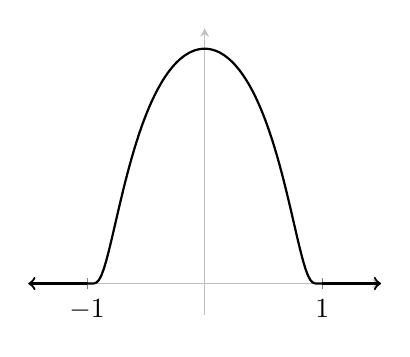
\begin{tikzpicture}
			\begin{axis}[
			xmin=-1.5,xmax=1.5,
			ymin=-0.05,ymax=0.4,
			ytick={0},
			xtick={-1,1},
			xticklabels={$-1$,1},
			yticklabels={},
			axis lines=middle,
			axis line style=lightgray,
			width=0.5\textwidth
			]
			
			
			\addplot[black,style=thick] expression[domain=-0.999:0.999,samples=100]{exp(-1/(1-x^2))}; 
			
			\addplot[black,style=thick,<-] expression[domain=-1.5:-1,samples=2]{0};
			
			\addplot[black,style=thick,->] expression[domain=1:1.5,samples=2]{0};
			\end{axis}
			\end{tikzpicture}
		\end{center}
		\caption{The graph of the function $\psi$ from \cref{canonical-bump}.}  \label{canonical-bump-graph}
	\end{figure}
\end{example}

\begin{exercise}
	For any $a < b$ in $\R$, construct a bump function $f : \R \to \R$ whose support is $[a,b]$. 
\end{exercise}

\begin{exercise}
	Let $F$ be a closed subset of $\R$. Construct a smooth function $f : \R \to \R$ which is zero on $F$ and nonzero outside of $F$. \begin{hint} Recall that the complement of $F$ is a countable disjoint union of open intervals (cf. \cite[theorem 6.17]{protter-morrey}). \end{hint}
\end{exercise}

\subsubsection*{Bridge functions}

Next up, we'll discuss an example of a ``bridge'' function.\index{bridge function@``bridge'' function} It will be constant on $(-\infty, -1]$, and also constant on $[1, \infty)$, but the values on these two intervals is different; and on $(-1,1)$, the function ``smoothly bridges the gap'' between the two values. 

In discussing this example, we will invoke the fundamental theorem of calculus,\index{fundamental theorem of calculus} even though we have not proved it (or even defined integrals, for that matter). If you're unhappy with using things you haven't proved, you can find rigorous discussions of integration in many places (eg, \cite[chapter 5]{protter-morrey}, \cite[chapter 6]{rudin}, etc). Alternatively, you might also be interested in \cite[chapter 3, example 12]{counterexamples}, which gives an example of a ``bridging function'' that involves no integrals (but does involve a double exponential). 

\begin{example} \label{bridge-function}
	Let $\psi$ be the bump function from \cref{canonical-bump}, and then consider 
	\[ \eta(x) = \int_{-1}^x \psi(t)\, dt. \]
	Then 
	\[ \eta'(x) = \frac{d}{dx} \int_{-1}^x \psi(t)\, dt = \psi(x) \]
	by the fundamental theorem of calculus. Thus $\eta$ is smooth, since $\eta' = \psi$ is smooth. Note moreover that $\eta$ is increasing, since $\eta' = \psi \geq 0$. Finally, it is clear from the geometric interpretation of integrals as ``area under the curve'' that $\eta$ is constantly equal to 0 for all $x \leq -1$ and that it is constantly equal to $\eta(1)$ for all $x \geq 1$. 
\end{example}

\begin{exercise} \label{constant-compact-zero-outside-neighborhood}
	For $a < b$ in $\R$, let $I = [a, b]$ and let $U$ be an open subset containing $I$. Prove that there exists a bump function $f : \R \to \R$ such that $f(x) = 1$ for all $x \in K$ and $f(x) = 0$ for all $x \notin U$. \begin{hint} 
	The characteristic function \[ \chi_I(x) = \begin{cases} 1 & \text{if } x \in I \\ 0 & \text{if } x \notin I \end{cases} \]
	is close to having all of the properties we want, but it's not smooth; it's clearly not even continuous. ``Bridge'' the discontinuities.\index{bridge function@``bridge'' function} \end{hint}
\end{exercise}

%TODO: Newton's method